\begin{savequote}[8cm]
  ``I have not failed. I've just found 10,000 ways that won't work.''
  \qauthor{Thomas Edison}
\end{savequote}
\makeatletter
\chapter{Methodology}


\section{Fourier Volume Reconstruction}
\label{FVRSectionA}

Here we present several techniques used to extract dense 3D reconstruction from image/video data. In the first section we describe techniques in addition to Fourier volume registration. These include the recovery of translation, y-axis rotation and scale information as well as a technique for the recovery of a so called 7 degrees of freedom transform. \\

We also list notable speed-ups for volume registration which reduce the amount of processing by over a third. After this, a full 3D reconstruction technique based on the principles of phase correlation is presented. Then we also present two novel reconstruction data representations which may be used to efficiently represent and fuse 3D reconstructions. Lastly, different sensor inputs are discussed and some conclusions are given about the usefulness of this technique in the context of these sensors is presented.

\subsection{Volume Registration}
Fourier volume Registration within the context of a 3D reconstruction procedure requires two frames of 3D data. These two frames may be input as any 3D representation: mesh, volume, point-cloud, SDF or in a compressed format (eg. Octree). However, the input must be converted to a 3D signal or volume representation prior to phase correlation. Moreover, the size of the volume should be cubic and the data should be scaled to fit. If the two frames are scaled un-evenly then the method must also be registered against scale. This section details some of these issues and more within the context of video sensor input from sensors.  \\
 

\subsubsection{Camera Translation}
\label{sec:PCForSLAM}
To describe camera translation, let's say a camera produces 3D scans of a scene from a particular pose. This may be performed implicitly (in the case of stereo or monocular depth estimation procedures) or explicitly (through the use of such sensors i.e-Microsoft Kinect, Asus Xtion Pro Live) and normalizes them into a 3D volume frames. If the camera captured frame 1, then moved 20 units to the left, before capturing frame 2, visualizing these frames in conjunction with each-other, it would appear the data was shifted to the right by $20$ units ($20\theta$ if the resolution of the 3D volume differs by a scale of $\theta$). If the volumes were to be registered (assuming no error), it would be found that the data from frame 1 to frame 2 had been translated by $T_{frame-1,frame-2} = [20,0,0]^T$, which can be performed using the translation matrix in equation \ref{eqn:TransRegMatrix}.

\begin{equation} \label{eqn:TransRegMatrix}
\left[
\begin{array}{cccc}
1 & 0 & 0 & 20 \\
0 & 1 & 0 & 0 \\
0 & 0 & 1 & 0 \\
0 & 0 & 0 & 1 \\
\end{array}
\right]
\end{equation}

The volume data has shifted in the opposite direction. Therefore to register the data, frame 1 may be transformed by the matrix in equation \ref{eqn:TransRegMatrix} to align it with frame 2. Conversely, the camera pose may be updated by adding $T_{frame-1,frame-2} \times -1$ to the camera's location.  \\

Generalizing this, we define a volume $V_1$ captured as the first frame and a second volume $V_2$ which is captured after moving the camera in a particular direction (up, down, left, right, forward or backward) scaled by a magnitude (a vector). The translation from $V_1$ to $V_2$, $(x,y,z)$ can easily be recovered via phase correlation. As described, the camera pose may be updated by $-1 \times (x,y,z) = (-x,-y,-z)$. \\

Here we step into the detail of phase correlation with deeper insight with respect to the superficial introduction from section \ref{Sec:SuperficialPCSection} and with a focus on 3D data and pose estimation. Firstly, we define the correlation measure process. Correlation in the context of signal processing measures signal shape similarity between two signals. \\

In this measure, large correlation values signify a greater similarity in terms of shape, where as a smaller value signifies the signals have very different shapes. Note, large negative values signify the shapes may be similar but mirrored. Following the doctrine of DSP, that all signals, no matter what dimension may be processed similarly with similar operations and measures, this technique can be applied to measure similarities between volumes.  \\

The measure of correlation between $V_1$ and $V_2$ can be found by shifting $V_1$ and $V_2$'s mean values to zero. By doing this, the mean value cannot affect the correlation measure. For example, if the first frame was captured in low light and the second in a brighter light. The resulting values for frame 2 may look like those from frame 1 in terms of values fluctuating about a mean, however the change in lighting may affect the voxel values by increasing them by a uniform value or scaling them by some scalar. Therefore, by subtracting the mean we place the signals in states where by their shape, rather than their raw values may be compared. The procedure can then be completed by summing the element-wise multiplication of $V_1$ by $V_2$. When $V_1$ has a positive voxel value (a voxel value above the mean) and so does $V_2$'s corresponding voxel in the same position, the multiplication value is positive, and this is summed into the correlation measure. This is the same situation as if both voxel values were negative (both below the mean). On the other hand, if one voxel value was positive and the other were negative, the correlation measure would be rectified accordingly. Equation \ref{eqn:CorrelationEquation} computes this correlation measure. 

\begin{equation} \label{eqn:CorrelationEquation}
\sum_{z=0}^{N}\sum_{y=0}^{N}\sum_{x=0}^{N}(V_1(x,y,z)-avg(V_1)) \times (V_2(x,y,z)-avg(V_2))
\end{equation}

As mentioned, correlation may be used to measure the similarity between two volumes' shapes. In the context of registration for 3D reconstruction algorithms, it can be used to measure the accuracy of a registration. Again using $V_1$ as frame 1 and $V_2$ as frame 2, given a supposed transform $T_{est}$ to register $V_1$ to $V_2$. The measure of registration may be defined as $correlate(T_{est}(V_1), V_2)$. The measure may be used to compare two registrations, possibly in order to select the better registration in terms of correlation measure. The two frames may be captured under different lighting conditions and the correlation measure will still be able to be used to select the best transform. \\


Within the framework of measuring camera pose, the cross-correlation algorithm may be used to measure the correlation values for each possible camera movement, and define the camera location as the location with the largest correlation value. This algorithm is shown in listing \ref{algorithm:CrossCorrelationAlgorithm}.

\begin{figure}
\begin{lstlisting}[language=c++,caption=Cross-Correlation based camera location estimation,label=algorithm:CrossCorrelationAlgorithm,mathescape,basicstyle=\ttfamily]
$V_1$ = CaptureFrame();
//shift camera
$V_2$ = CaptureFrame();
$highest-correlation$ = $infty $;
camera-location = $[0,0,0]$;
for($z$ in $[0,N]$){
  for($y$ in $[0,N]$){
    for($x$ in $[0,N]$){
      $V_{temp}$ = translate(V_1, x, y, z);
	  $tempMeasure$ = correlate($V_{temp}$, $V_2$);
	  if($tempMeasure$ > $highest-correlation$){
	    $highest-correlation$ = $tempMeasure$;
		$camera-location$ = $[-x,-y,-z]$;
	  }		
	}
  }
}
\end{lstlisting}
\end{figure}

Cross correlation is typically used in signal processing to compute the best alignment for two signals. In this context it has been used to compute the best camera location change, notice in the algorithm the $camera-location$ variable is set to be the inverse of the translation amount being tested ($[-x,-y,-z]$). Again this is because when the optimal translation value aligning frame 1 to frame 2 is defined as vector $v$, then the camera location change is equivalent to the inverse. The cross-correlation function in this context may be thought of as an exhaustive optimization procedure which optimizes the camera location change (equation \ref{eqn:CrossCorrelationEquation11}) in terms of the correlation function.  \\

\begin{equation} \label{eqn:CrossCorrelationEquation11}
correlate(translate(V_1, x,y,z), V_2)
\end{equation}

The range of camera location vectors to test is dependent on the dimensions of the raw 3D input data. If the data is scaled to fit an $N^3$ space, as is a requirement when using Fourier based techniques, the camera location values along the x, y and z axis would range between 0 and $N$. To compute the optimal camera location change using the phase correlation method would therefore have complexity $N^3$. There are $N^3$ values to test, and the correlation function must be called for each iteration with a complexity also equivalent to $N^3$, $N^3 \times N^3 = N^6$. This is significantly complex, even for smaller volume sizes. Note that the smaller the volume size, the faster the algorithm, however the more quantized the original data is. The more the input data is quantized, the more the camera location change estimates will be restricted in terms of precision. Accuracy will also be affected as quantization introduces unwanted effects of its own. The answer is to use the properties of the Fourier transform to speed up the process.  \\

\begin{figure}[!htb]
\centering
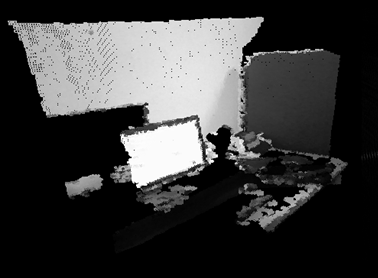
\includegraphics[width=6cm]{images/methodology/FVR/capFrameOriginal}
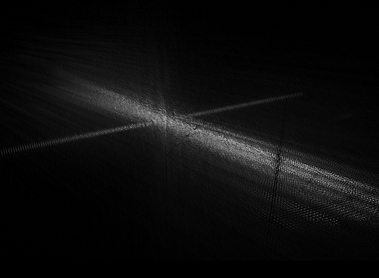
\includegraphics[width=6cm]{images/methodology/FVR/capFrameMagFFT}
\caption{Left: Captured 3D frame, Right: Magnitude values in the frequency domain of the captured 3D frame}
\label{fig:FrequencyDomainExample}
\end{figure}
 
The 3D Fourier transform transforms a volume from the 3D spatial domain into the 3D frequency domain (see figure \ref{fig:FrequencyDomainExample}). The frequency domain is a complex valued volume made up of sinusoids. Each voxel in the frequency domain represents the magnitude, phase and direction of a wave. These properties are important for computing camera pose as shall be discussed upcoming sections. An efficient software implementation of the Fourier transform named the Fast Fourier Transform (FFT) is able to compute the frequency domain given N-dimensional data. \\

Exploiting the properties of the FFT and the frequency domain, cross correlation may be carried out efficiently in order to compute the optimal camera location change between frames. As in the 2D approach, this algorithm is named phase correlation and is a popular approach in 2D image processing to align two images. Applied to two 3D frames captured by sensors (or partially generated via software) it may also be used to register the frames for 3D reconstruction as well as compute the translation part of the camera pose change for SLAM algorithms. This procedure is defined here as a function named $PhaseCorrelation$ (Eq. \ref{eqn:PC_basic}). This function takes two frames (3D volumes) as input and returns the best translation alignment between them in terms of maximizing correlation.  \\

\begin{equation} \label{eqn:PC_basic}
T(x, y, z) = PhaseCorrelation(V_x, V_y)
\end{equation}

The $PhaseCorrelation$ consists of 4 steps. In the first step the two captured 3D frames $V_1$ and $V_2$ are transformed into the frequency domain using the Fast Fourier Transform. This computes two new volumes $F_{1_{x,y,z}} = FFT(V_1)$ and $F_{2_{x,y,z}} = FFT(V_2)$. Applying the Fourier Shift Theorem to the context of camera pose estimation, if frames $V_1$ and $V_2$ are separated by some camera translation, then $F_{1_{x,y,z}}$ and $F_{2_{x,y,z}}$ will have phase values shifted relative to each-other. The normalized cross power spectrum (equation \ref{eqn:PHCOR_eq}) of the two complex valued Fourier spaces may then be used to find the camera translation change. The normalized cross power spectrum of $F_{1_{x,y,z}}$ and $F_{2_{x,y,z}}$ is another complex valued volume of the same size. \\

\begin{equation} \label{eqn:PHCOR_eq}
F_{3_{x,y,z}} = \frac{F_{1_{x,y,z}} \circ F_{2_{x,y,z}}^*}{ | F_{1_{x,y,z}} \circ F_{2_{x,y,z}}^* | }
\end{equation}

In equation \ref{eqn:PHCOR_eq}, $\circ$ is an element-wise multiplication and $|x|$ is the magnitude function or absolute value function. The Inverse Fast Fourier Transform ($IFFT$, $FFT^{-1}$) may then be used on the output of the normalized cross power spectrum volume to produce a phase correlation surface. The peak value on the phase correlation surface represents the optimal value of the correlation function applied to the two original real valued 3D frames. Therefore the $PhaseCorrelation$ procedure is equivalent to the cross correlation procedure, but rather than being complexity $N^6$, phase correlation reduces the complexity to approximately $6N^3 \times Log(N)$. \\


Due to the nature of camera capture, if the camera is translated by some vector before the capture of the next frame. Then the first frame contains data which the second frame does not, conversely, the second frame will capture some other data which is not present in the first frame (unless the camera was not moved). The parts of the 3D frames which do not overlap cause noise on the phase correlation surface. This makes it more difficult to decipher the location of the peak. There may be several peaks to choose from, or no clear peak. The nature of computing the Discrete Fourier Transform also affects this. The Discrete Fourier Transform assumes the output Fourier space is an infinitely repeating signal. The cross correlation procedure on the other hand does not assume this, so therefore the phase correlation surface may be affected. The solution adopted by many is to filter the volumes prior to transforming into the frequency domain. This can be done using a Hanning window function (equation \ref{eqn:HanningFunction}). This function can be used to filter edge effects prior to computing the Fourier transform which helps to reduce noise on the phase correlation surface. \\

\begin{equation} \label{eqn:HanningFunction}
Hanning(x) = \frac{1}{2}(1 - cos\left(\frac{2\pi x}{\frac{N}{2} - 1}\right)
\end{equation}

Noise on the phase correlation surface may also be present if other types of transforms are. In this case, the true camera translation may be lost. Therefore, camera pose/rotation must be computed prior to computing the camera translation. Other artefacts which may produce noise on the phase correlation surface include moving objects. If an object is present in one scene and not the other, it will cause some noise to be present in the phase correlation surface, making finding the peak more difficult but not impossible. Alternatively if there is an object whose location is changed between frames, the same thing may happen. The phase correlation procedure should be robust to these artefacts already but filtering approaches may also prove useful in selecting the correct peak which optimizes the translation used to register the 3D camera frames. \\

\subsubsection{Camera Rotation and Zooming}
\label{Sec:RoteZoomingSection}
SLAM and 3D reconstruction algorithms must compute both the camera location changes as well as camera pose. SLAM must compute this pose to track the camera, 3D reconstruction methods may simply register the data for integration or compute the camera pose prior to alignment and integration. Computing this involves estimating the camera's post change (rotation) from one frame to another. This may take the form of a $4 \times 4$ rotation matrix or the explicit magnitudes of rotation for each axis in a pre-determined order. These two formats may be converted between each other. The pose may also be represented by three axes (three orthogonal vectors) which represent the coordinate space of the camera. \\

Another transform not covered often in 3D reconstruction literature is that of scale. Given a single camera moving in a 3D space, scale is of no concern. However, if frames are zoomed or data is computed across sensors, scale factors may be unknown. For example, if an RGB-D image is captured as frame 1 and a second is captured as frame 2, but frame 2 is zoomed (scaled) prior to projection then the data may still be registered if scale may also be recovered. Alternatively if frame 2 is captured by another sensor or software system and is projected at a different scale, then this scale should also be recovered. The recovery of scale could be considered most important in the case of monocular 3D reconstruction. Here, the fundamental matrix may be used to calibrate camera frames. Once calibrated, stereo methods may be used to extract dense depth information for each frame. The problem with this technique is that depth is relative but not to scale across multiple frames. If the scale could also be recovered during the camera pose estimation procedure it would eliminate the need for more advanced methods of optimization. \\ 

Phase correlation alone cannot register against camera rotation. An important part of SLAM is the ability to recover 3D camera pose, and a fundamental part of 3D reconstruction is to align dense depth data against as many camera movements as possible. Therefore we propose using an extension of the popular rotation and scale recovery procedure from 2D registration research to perform camera rotation change estimation as well as align frames which have been zoomed or scaled to fit the volumetric space. \\

Using this technique, which is comprised of a few spatial transformations and phase correlation, a single axis of rotation may be recovered. The axis chosen is integrated into the spatial transformation part of the procedure. Since most scenes would be captured by moving around a room and rotating the camera to look at the areas within the scene directly around the user and camera, we have designated the y-axis of rotation as the most important axis to recover. Additionally, vehicles (with dash mounted cameras) and robots typically keep the camera steady and perform movements and rotations about the y-axis. This technique's application to 3D reconstruction is novel in itself, but a completely novel technique named FVR3D is presented in this work for recovering all 3 axes of rotation using Fourier techniques, this is discussed in section \ref{FullRecovery3DSection}. FVR3D makes use of the rotation and scale estimation procedure discussed here.  \\


Given two frames captured as 3D volumes, $V_1$ and $V_2$, where $V_2$ is captured by a second camera at a different location, pose (about the y-axis) and has data projected differently prior to both systems submitting data for registration and integration into a single global 3D reconstruction. From the perspective a registration system, the data in frame 2 has been transformed by translation vector $t = [t_x, t_y, t_z]$, rotation factor $\theta$ and scale $\varphi$. The procedure to recover these values makes use of several properties of the Fourier transform and the frequency domain. One important property is that, the magnitude of the frequency domains of both $V_1$ and $V_2$ are related differently to the raw data from the frames alone. The magnitudes are related by the same rotation factor $\theta$ and scale factor$\varphi$, but these transforms occur about the origin at the center of the magnitude volumes, rather than at locations which depend on the translation factor $t$. In this way, the translation factor can be ignored and the rotation and scale factors can be recovered separately. \\


\begin{figure}[!htb]
\centering
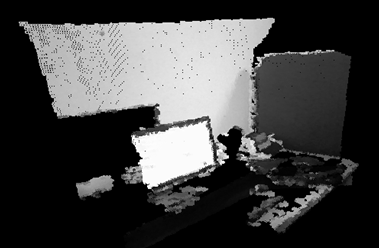
\includegraphics[width=6cm]{images/methodology/FVR/capFrameA}
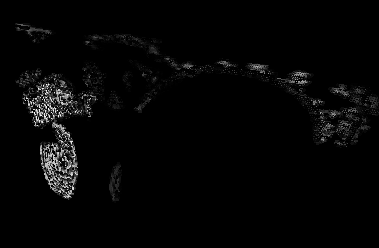
\includegraphics[width=6cm]{images/methodology/FVR/capFrameLogPolar}
\caption{Left: Captured 3D frame, Right: Log-Polar Transform of the captured 3D frame}
\label{fig:LogPolarTransform3DExample}
\end{figure}

This procedure recovers the camera rotation as well as any scale factor which may be present independent to any translation effects. Therefore, once the rotation and scale factors have been recovered, the translation parameters may be estimated using the 3D phase correlation procedure described in section \ref{sec:PCForSLAM} as an additional step. This procedure starts by applying a Hanning windowing function to both volume frames. As mentioned the Hanning window function is used to counter the noise generated by the Fourier transform. This noise occurs because the discrete frequency domain is assumed to be infinity repeating when in practical computer algorithms the space is treated as singular occurring structure surrounded by finite empty space. This unavoidable assumption makes some operations on the frequency domain erroneous. The function for the Hanning window was given in equation \ref{eqn:HanningFunction}, the scalar for each voxel in frames may be computed for each point $[x,y,z]^T$ via equation \ref{eqn:Hann}. The use of this filtering is especially important in computing the rotation and scale parameters. \\


\begin{equation} \label{eqn:Hann}
\scriptstyle
HW_{x,y,z} = \frac{1}{2}\left(
1 - cos \left(
\frac{2\pi
\left(
\sqrt{\left(\frac{N}{2}\right)^3} -
\sqrt{
\left(x-\frac{N}{2}\right)^2 + \left(y-\frac{N}{2}\right)^2 + \left(z-\frac{N}{2}\right)^2
}
\right)
}
{2\sqrt{\left(\frac{N}{2}\right)^3} - 1}
\right)
\right)
\end{equation}

The translation separating the camera frames must be removed from the equation prior to estimating the rotation and scale. As mentioned, the magnitude of the frequency domain is independent to the effects of translation. So, the magnitude of the frequency domains of both frames are taken, $M_1 = |FFT(V_1)|$, $M_2 = |FFT(V_2)|$. The zero frequency, which is at the corners of the volume (because the discrete frequency domain is assumed to be circularly repeating infinitely) must be transformed to the center of the volume. In this way, any rotation or scaling occurs about the center of the volume. Then, both $M_1$ and $M_2$ are filtered using an element-wise log function. The frequency domain contains larger values around the zero mean and low frequency areas and smaller values around the higher frequency areas, but for the purposes of computing the camera rotation and any possible scale factor, all frequencies should be treated equally. The element-wise log function therefore suppresses the lower frequency values bringing the higher frequencies up to a similar level. \\

Given these new volumes, $M'_1 = Log(M_1)$, $M'_2 = Log(M_2)$, a geometric transform named the log-spherical transform is used on both $M'_1$ and $M'_2$. The log-spherical transform function re-arranges the input data in such a way, that any y-axis rotation becomes x-axis translation and any scaling becomes z-axis translation. Equation \ref{eqn:Log_Spherical} shows the log-spherical space coordinate $(X_{log-spherical}, Y_{log-spherical}, Z_{log-spherical})$ for a given $(x,y,z)$ euclidean space coordinate. This encompasses the effects of the log-spherical transform. \\


The output x coordinate, $X_{log-spherical}$ in the log-spherical transform centers the input x and y coordinates about the centre of the volume and uses the atan trigonometric function to obtain the angle in degrees the point is around the y-axis. This is scaled to the full size of the volume via scalar $\frac{N}{360}$. The result is that data at different angles about the y-axis are grouped by their particular angle linearly along the output x-axis. The output y coordinate $Y_{log-spherical}$ is also centered about the volume center and is put through the cosine function. This gives the angle in degrees about the secondary axis (x rotational axis). The degree between 0 and 180 is then mapped to the range $[0-N]$ using the scalar $\frac{N}{180}$. The y coordinate can be passed to the cosine function directly because it is known that the x rotational angle can be computed as the cosine function of the dot product between the input point, $[x,y,z]^T$ and the vertical axis $[0,1,0]^T$ which results in $x \times 0 + y \times 1 + z \times 0 = y$. \\

The output z, $Z_{log-spherical}$ coordinates encompasses the scale information of the input coordinate. First the distance between the input coordinate and the center of the volume is computed. This is placed through a log function, the log function compresses the distance such that any scaling relationship between distances becomes a relationship of addition, or in this case volume translation along the z-axis. This is then mapped using the scalar $\frac{N}{log\left(\frac{N}{2.56}\right)}$. This mapping is used so that scales within the range $[2.56^{-1}, 2.56]$ may be registered. Increasing this range too much results in decreased precision and possibly a decrease in accuracy or an inconclusive registration result. \\


\begin{equation} \label{eqn:Log_Spherical}
\begin{split}
X_{log-spherical} & = \frac{atan\left(
\left( x-\frac{N}{2} \right) \times
\left(y-\frac{N}{2}\right)^{-1}
\right)N}{360}\\
Y_{log-spherical} & = \frac{acos\left(
y-\frac{N}{2}
\right)N}
{180} \\
Z_{log-spherical} & =\frac{log\left(
\sqrt{\left(x-\frac{N}{2}\right)^2+\left(y-\frac{N}{2}\right)^2+\left(z-\frac{N}{2}\right)^2}
\right)N}{log\left( \frac{N}{2.56} \right)} \\
\end{split}
\end{equation}

The log-spherical transforms of $M'_1$ and $M'_2$ are then related by translation. The translation relationship describes the camera rotation and the scale factor separating both of the original frames. The exact translational differences can easily be recovered using phase correlation. The resulting peak location from the phase correlation procedure, $(x_{M'},y_{M'},z_{M'}) = PhaseCorrelation(M'_1, M'_2)$ is used to estimate the rotation and the scale. The phase correlation surface of these two volumes is often very noisy. It is usually noisier than phase correlating data from the spatial domain. Filtering techniques may be used to alleviate this issue. If multiple peaks are detected, the rotation and scale may also be tested for each candidate peak. The rotation $\theta$ and scale factor $\varphi$ separating the two original frames, $V_1$ and $V_2$ can then be computed using the peak values on the phase correlation surface, $(x_{M'},y_{M'},z_{M'})$. The functions to compute $\theta$ and $\varphi$ are given in equation \ref{eqn:ROTATIONSCALEFROMXM}. \\
 
\begin{equation} \label{eqn:ROTATIONSCALEFROMXM}
\begin{split}
\theta & = \frac{-360x_{M'}}{N}\\
\varphi & = e^{
-\left(
2.56^{-1}N
\right)z_{M'}N^{-1}
}
\end{split}
\end{equation}

The $(x_{M'}$ coordinate is mapped to a unit number in the range $[0,1]$ and is scaled by $-360$ resulting in $\theta$, the angle of rotation which may be used to align the frames. The $z_{M'}$ coordinate is also mapped to a unit number, it is then scaled by $\frac{N}{256}$ in order to align the result prior to inverting the log function effects. The value is negated also, this gives the relationship relative to frame 1 rather than frame 2. Finally, the log function is reversed using the exponential function. The resulting rotation matrix may be formed as in equation \ref{eqn:RoteRegMatrix}. This conjuncted matrix first transforms the center of the volume to the origin and then rotates it by $\theta$, then transforms it back to the center of the volume. \\

\begin{equation} \label{eqn:RoteRegMatrix}
\left[
\begin{array}{cccc}
1 & 0 & 0 & \frac{N}{2} \\
0 & 1 & 0 & \frac{N}{2} \\
0 & 0 & 1 & \frac{N}{2} \\
0 & 0 & 0 & 1 \\
\end{array}
\right] \times
\left[
\begin{array}{cccc}
cos(\theta) & 0 & sin(\theta) & 0 \\
0 & 1 & 0 & 0 \\
-sin(\theta) & 0 & cos(\theta) & 0 \\
0 & 0 & 0 & 1 \\
\end{array}
\right] \times
\left[
\begin{array}{cccc}
1 & 0 & 0 & -\frac{N}{2} \\
0 & 1 & 0 & -\frac{N}{2} \\
0 & 0 & 1 & -\frac{N}{2} \\
0 & 0 & 0 & 1 \\
\end{array}
\right]
\end{equation}

The resulting scaling matrix is formed similarly (equation \ref{eqn:ScaleRegMatrix}) by transforming the volume center to the origin, scaling the geometry and then transforming the data back to the center of the volume. The resulting matrix to un-do both the scale and rotational effects of the camera movement can therefore be computed as the scale matrix multiplied by the rotational matrix, $SR_{matrix} = S_{matrix} \times R_{matrix}$. \\

\begin{equation} \label{eqn:ScaleRegMatrix}
\left[
\begin{array}{cccc}
1 & 0 & 0 & \frac{N}{2} \\
0 & 1 & 0 & \frac{N}{2} \\
0 & 0 & 1 & \frac{N}{2} \\
0 & 0 & 0 & 1 \\
\end{array}
\right] \times
\left[
\begin{array}{cccc}
\varphi & 0 & 0 & 0 \\
0 & \varphi & 0 & 0 \\
0 & 0 & \varphi & 0 \\
0 & 0 & 0 & 1 \\
\end{array}
\right] \times
\left[
\begin{array}{cccc}
1 & 0 & 0 & -\frac{N}{2} \\
0 & 1 & 0 & -\frac{N}{2} \\
0 & 0 & 1 & -\frac{N}{2} \\
0 & 0 & 0 & 1 \\
\end{array}
\right]
\end{equation}

If frame 1, $V_1$ is then transformed by scale-rotation matrix $SR_{matrix}$, the resulting volumes are separated only by translation. The translation matrix separating them may then be computed using phase correlation. The result of this procedure is that the rotation factor $\theta$, the scale factor $\varphi$ and the translation factors $x$, $y$ \& $z$ have all been recovered. Given the translation matrix $T$ formed by the translation factors $x$, $y$ \& $z$, the full registration matrix aligning frames $V_1$ and $V_2$ may be computed as, $M_{T,\varphi,\theta} = T \times SR_{matrix}$. $M_{T,\varphi,\theta}$. This matrix can be used to align frame 1 to frame 2 prior to integration. Alternatively frame 2 may be aligned with frame 1 by transforming it by $M_{T,\varphi,\theta}^{-1}$. \\

The camera pose relationship between frame 1 and frame 2 is also now known. Given the camera coordinate axes in frame 1, $Forward \in R^3$, $Right \in R^3$, $Up \in R^3$ the coordinate space for the camera in frame 2 may be computed by adjusting these axes by the registration matrix $M_{T,\varphi,\theta}$. Once the camera pose is known, the camera may be tracked by repeating the process between successive frames, the resulting dense 3D data may then be integrated to create the complete 3D reconstruction. Alternatively, the dense 3D data may be projected and integrated directly resulting in the output 3D reconstruction. \\

\subsubsection{Conclusion}

In this section, the volume registration method is applied to 3D pose estimation. In the next section this is extended into a full 3D reconstruction algorithm. Experiments in sections \ref{Sec:FVRSOTA,Sec:CamTransTrackExp}
show that this method is capable of reconstructing scenes accurately using different sensors whilst being robust to noise. 

\subsection{Fourier Volume Reconstruction}

Section \ref{Sec:VolumeRegistrationSection} described techniques to register camera frames which have been projected to three dimensions. As mentioned, these frames may be registered with respect to the most common type of camera pose transform, y-axis rotation, as well as camera movement. In addition, scale may be registered. For frames which have been projected differently or frames in which depth is computed relative to each frame, such as per frame depth computed in monocular view situations, scale is an important transformation to register against. This is especially true since most existing methods perform simple rigid movement camera pose registration. \\

This section integrates the phase correlation method into a full 3D reconstruction algorithm named Fourier Volume Registration (FVR). This algorithm may also be used to perform SLAM and it may be applied to input data in which depth is not projected at correct scale between frames. The input required for this method is a list of colour RGB images, each with a depth component. The data may be generated via an RGB-D active camera or computed implicitly using a stereo camera set-up or calibrated monocular set-up. \\

Results for the FVR method are presented in sections \ref{StereoSOTA}, \ref{ActiveSOTA}, \ref{Sec:MonocularSOTA} and \ref{Sec:CamTransTrackExp} and show the FVR method is capable of accurate 3D reconstructions whilst being robust to noise. In some experiments, it also outperforms the current state-of-the-art methods from the literature. Details on how the Fourier Registration methods described in section \ref{FVRSectionA} are integrated to create the FVR algorithm are presented in the following sections. \\


\subsubsection{Pipeline}

\label{sec:FVRPipelineSect}

In Figure \ref{fig:PIPELINENo1} a pipeline for the FVR registration method is shown. This is a high-level pipeline for the recovery of scale, y-axis rotation and translation. Many of the operations may be performed using GPU processing techniques. Signal Processing methods are very common, many hardware devices exist which can execute these algorithms which are used by the FVR method. \\

Two volumes, $Volume_1$ and $Volume_2$ are both first put through a Hanning window function, these operations may be performed in parallel. This process multiples each voxel by a scalar which may be computed entirely based on location or a 3D lookup table. Each Hanning window operation may also be performed on the GPU or using another parallel programming technique such as multi-threading. \\

Next, using the FFT the magnitude of the Discrete Fourier Transform is computed. The 3D FFT is a common operation which is implemented on most General Purpose Graphics Processing Units (GPGPUs). The 3D FFT operations on the GPGPUs produce the real and imaginary components of the frequency domain, but an additional GPU operation may be used to compute the magnitude values based on the real and imaginary values. Again this operation is easily extended to parallel processing platforms and both volumes may be transformed in parallel. \\

The $Log(x)$ function is also a per voxel operation which may be computed in a parallel processing platform and both volumes may be transformed in parallel. The log-spherical transform may be computed for each volume at the same time and is also inherently parallel. Additional memory requirements must also be met as both input and output volumes must be simultaneously kept in memory. \\

\begin{figure*}[!htb]
\centering
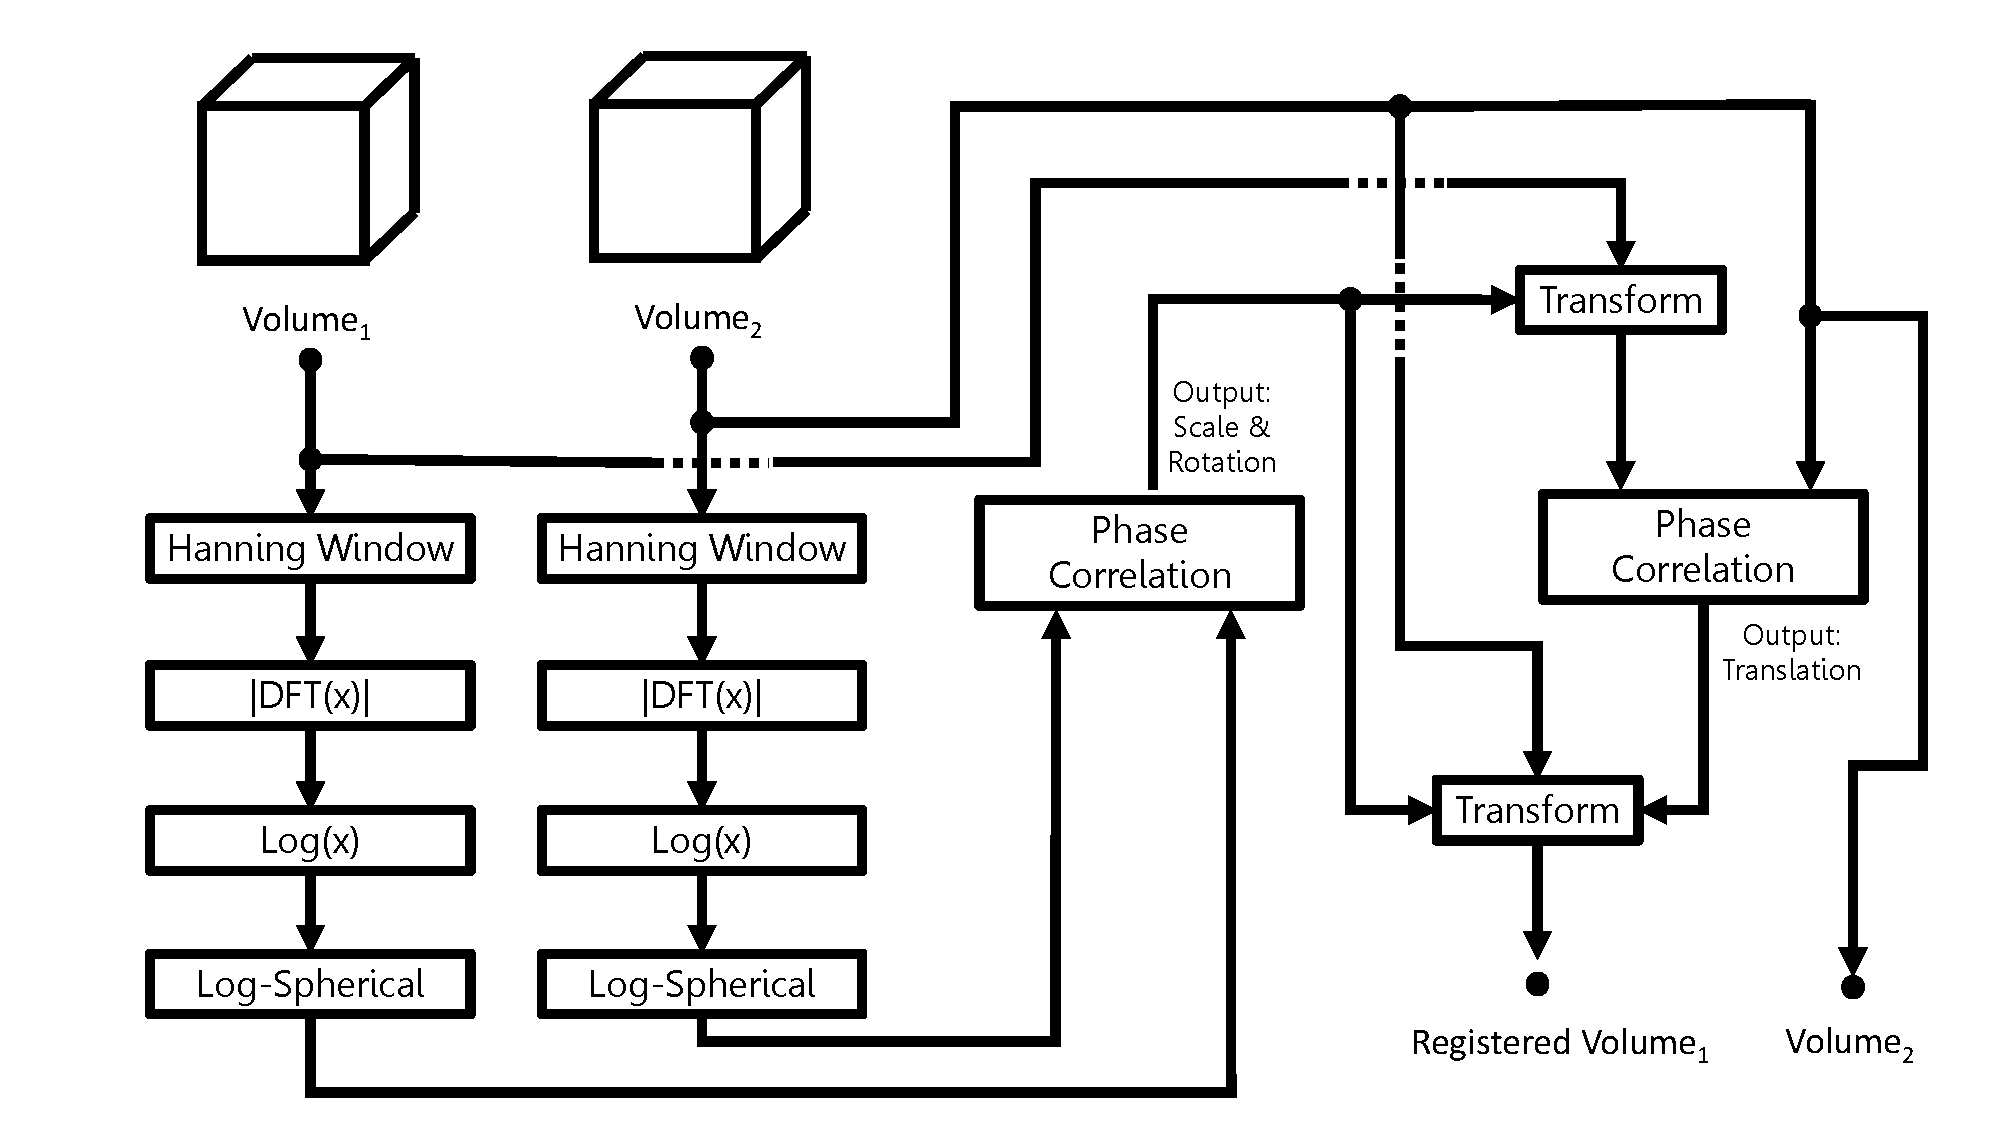
\includegraphics[width=5.0in]{images/ch2/pipeline2}
\caption{System Diagram for Registration Process}
\label{fig:PIPELINENo1}
\end{figure*}


The phase correlation operation is made up of multiple FFTs and their inverse, as well as computing the cross power spectrum between two volumes. All these operations may be performed on GPGPUs. Searching for the output peak is, however, a sequential process. Parallel techniques, such as reduction, may be used but the performance gain is minimal for volumes of size $256^3$. \\

Transforming the input volume is another process which may be performed using parallel techniques. The final phase correlation procedure is also parallel in nature apart from the peak value search on the phase correlation surface which is a sequential process. \\



\subsubsection{Algorithm}

Using the registration pipeline to compute the relationship between two frames, a SLAM and 3D reconstruction algorithm may be formulated. This algorithm can construct dense 3D reconstructions whilst simultaneously computing relative camera pose estimates. \\

 
The overall algorithm is presented in Listings \ref{algorithm:PCSLAMNo1}. In the first line, the first frame is read as an RGB-D image into variable $f_1$. This RGB-D image is projected into a 3D point cloud representation using a projection function. The point cloud data for this first frame is then integrated into an automatically expanding occupancy grid representing the global 3D reconstruction output variable named $GlobalReconstruction$. \\

An accumulation matrix, $M$, is used to formulate transforms for each frame read in. It is used by the algorithm to integrate frames directly into the output global reconstruction. Two variables, $Camera_{location}$ and $Camera_{pose}$, are used to represent the camera location and pose information. The pose contains three vectors representing the camera space within the world space. A list of the camera locations and poses is referred to by the $Cameras$ variable. Each element in this list is a camera location and pose pair. \\

\begin{figure}
\begin{lstlisting}[language=c++,caption=Phase Correlation Based SLAM Algorithm,label=algorithm:PCSLAMNo1,mathescape,basicstyle=\ttfamily]
$f_1$ = ReadFrame();
$PointCloud$ = project($f_1$);
$GlobalReconstruction$.integrate($PointCloud$)
$M$ = IdentityMatrix();
$Camera_{location}$ = $[0, 0, 0]^T$;
$Camera_{pose}$ = $[[1, 0, 0]^T,[0, 1, 0]^T,[0, 0, 1]^T]$;
$Cameras$ = $\left[\left[Camera_{location}, Camera_{pose}\right] \right]$;
while(more frames){
	$f_2$ = ReadFrame();
	$points_1$ = project($f_2$);
	$points_2$ = project($f_1$);
	$V_1$ = Voxelize($points_1$);
	$V_2$ = Voxelize($points_2$);
	$(\theta, \varphi, t_x, t_y, t_z) = VR_{\theta \varphi t_x t_y t_z}(V_1, V_2)$;
	$Temp = $TransformMat($(\theta, \varphi, t_x, t_y, t_z)$);
	$M = M \times Temp$;
	$points_1$ = Transform($points_1$, $M$);
	$GlobalReconstruction$.integrate($points_1$);
	$Camera_{location}$ = $Temp^{-1} \times Camera_{location}$;
	$Camera_{pose}$ = $Temp^{-1} \times (Camera_{pose} + Camera_{location})$;
	$Camera_{pose}$ = $\frac{Camera_{pose} - Camera_{location}}{Camera_{pose} - Camera_{location}}$;
	$Cameras.add(\left[Camera_{location}, Camera_{pose}\right])$;
	$f_1$ = $f_2$;
}
\end{lstlisting}
\end{figure}

The algorithm iterates over each frame pair which must be registered and integrated. Each iteration begins by reading in a new frame. This is pointed to by variable $f_2$. Next, both $f_1$ and $f_2$ are projected into point clouds named $points_1$ and $points_2$ respectively. The Fourier Volume Reconstruction method requires the frames be integrated into 3D volumes, so the Voxelize function is used to integrate the points and colour information into volumes. \\

The FVR method works with either integrated greyscale information based on the RGB data, or with raw binary occupancy values. The use of RGB data may have slight performance implications. Many computer vision algorithms prefer to work in greyscale, especially feature matching methods. This is often due to a combination of complexity and performance reasons. Whilst colour information does improve accuracy, it is considered to be minimal relative to savings made in terms of computational complexity by processing greyscale data alone. \\

Integrating the colour information for use in the FVR method does not incur any performance penalty. The only shortcoming of using the extra colour information to increase accuracy is the loss of the ability to work in total darkness using RGB-D sensors. \\

As mentioned in the literature, the Kinect Fusion technique only makes use of depth information which is obtained via an active camera (the Kinect). In this way it can effectively work in the dark. If the FVR method uses colour information integrated directly, and the colour components do not pick up any light, the method will fail. Whether or not colour information is present can be easily detected and because FVR also works by simply registering occupancy volumes, it can switch over to this method upon detecting that no colour (visible light) information is available. \\

Once the volumes are reconstructed, the rotation, scale and translation factors may be computed using the pipeline discussed in section \ref{sec:FVRPipelineSect}. A transformation matrix, $Temp$, may then be created from these values. Such a matrix was presented in section \ref{FVRSectionA}. $M$ is then replaced by itself multiplied by the computed transformation matrix $Temp$. In this way, $M$ can be used to accumulate previous registrations. \\

The $points_1$ point cloud is then transformed by the newly computed $M$. The point cloud can then be integrated into the global reconstruction. Next, the camera location and pose list must be updated. The camera location is adjusted by the inverse of the newly computed $Temp$ matrix. As previously mentioned, the camera transforms will be inversely related to the registration transforms. \\

The camera pose is also updated, by adjusting the axes relative to the camera location using the $Temp$ matrix. The camera pose vectors are then normalized and added into the list of camera locations and poses. Finally, $f_1$ is set to $f_2$. In this way, the algorithm can repeat with $f_1$ as the previous input frame. \\  



\subsubsection{Integration}

The integration procedure used with this technique is the common global voxel integration method. An automatically expanding volume is used to store the global 3D reconstruction. Given the algorithm described above, the output global reconstructed volume must take in point cloud data, and integrate it into the volume. \\

The algorithm proposed does not make use of loop closure. Many recent techniques also forgo the use of this procedure, especially if they integrate globally. The FVR method can also be easily adjusted by changing the last line of the algorithm. Rather than simply setting $f_1$ to $f_2$, $f_1$ may be set to the volume extracted by sampling the global reconstruction into a volume based on the most recent camera location and pose computed. This way, loops may be detected by registering upcoming frames globally. \\


\subsubsection{Limitations}

The FVR method is capable of registering 3D pose data and in turn can generate accurate, high quality 3D reconstructions. However, it is limited to a single axis of rotation (the y-axis). The FVR method was tested and remains robust to up to 10 degrees of rotation along the other axes, but it is still not able to register all 3 axes of rotation. To move past this limitation whilst retaining the robustness and accuracy of the technique, a novel extension named FVR-3D is proposed in section \ref{FullRecovery3DSection}. Both the FVR method and the FVR-3D algorithm are tested empirically in Chapter \ref{ch:Experiments} and results show they outperform other algorithms from the literature in terms of 3D pose estimation and 3D reconstruction. \\
\subsection{Monocular FVR}

During experiments, it was found that MVVR (FVR applied to monocular camera sensor data) had considerably less accuracy and robustness than the other FVR methods (FVR, FFVR and FVR-3D). Additionally, we found that MVVR was less robust to rotational transforms. This is due to the fact that depth maps produced by monocular sensor methods, such as optical flow, do not produce sufficiently accurate and reliable depth maps. Results from stereo and active camera tests suggest that this is due to the reduction in accurate and precise depth data generation. \\

Nevertheless, to evaluate the performance of the MVVR method, quantitative experiments were performed on the Kitti Vision Benchmark Data Set. In these experiments, the MVVR method was compared with methods from the literature including FM2D, FM3D. ICP and PCA. Each depth map was projected into volume sizes of $256^3$ for processing by the rest of the MVVR method (the FVR part). To generate the depth maps, a local 2D block matching method was used. Kernel sizes used in the correlation procedure were $3 \times 3$ in size with a search area size of $21 \times 21$. The sizes of the kernel, search area and volume sizes were all chosen empirically. \\

Depth maps computed using the block matching method are only estimates of true scene depth. Therefore, resulting projections are not accurate. These projections, however, are still good enough to produce reconstructions. Registration of these inaccurate projections is difficult due to the amount of noise in the data. Figure \ref{fig:lidarVSMono} shows the noise contrast between depth maps produced by a LIDAR and a monocular block-matching system. \\

\begin{figure}[!htb]
\centering
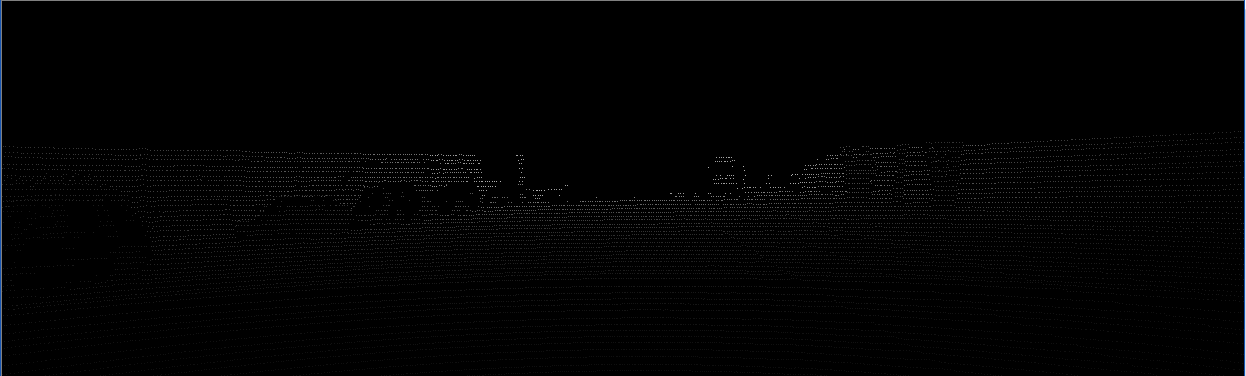
\includegraphics[width=2.9in]{images/methodology/FVR/mono/color}
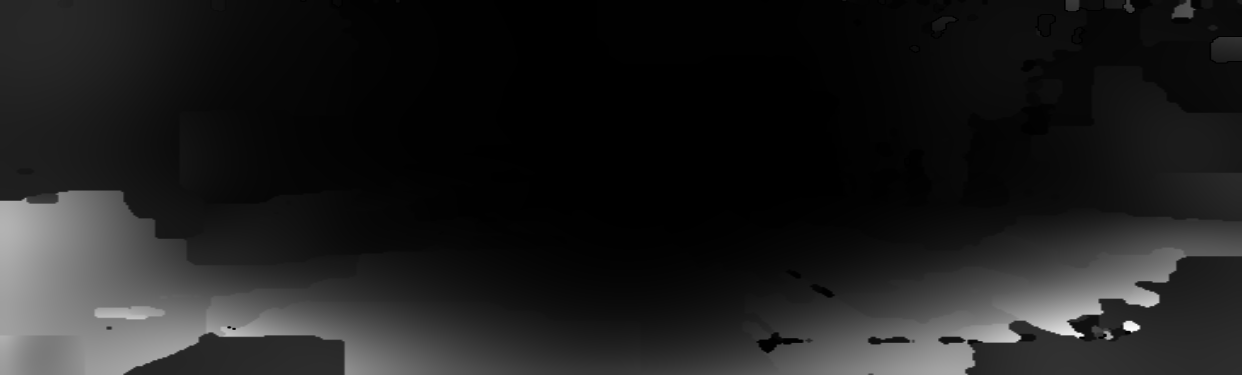
\includegraphics[width=2.9in]{images/methodology/FVR/mono/depth}
\caption{Left: Ground Truth Depth Map Computed Using a LIDAR System, Right: Depth Map Computed Using a Monocular Method}
\label{fig:lidarVSMono}
\end{figure}


Results on the Kitti Benchmark 0001 Sync data set are shown in Table \ref{table:MVVRQuantitativeExperimentResults}. In these results, ICP outperformed the other methods, with each algorithm having larger errors due to the inaccurate depth maps. Here, FVR achieved the best result ~29.25 \% of the time. Compared to results in Table \ref{tab:kittidata0001sync}, the MVVR method was less competitive than ICP. Due to the low-quality projections, FM2D and PCA failed were not able to register every frame. Most of the algorithms had incorrectly registered frames at some point.

\begin{table}[t]
\centering
\caption{Reconstruction Errors for the Kitti Data 0001 Sync Data Set Using Monocular (RGB) Input Only}
\begin{tabular}{ccc}
\hline
\textbf{Algorithm} & \textbf{Median Error $\times$ 1000} & \textbf{\% best results}\\ \hline
FM2D	& 3742.4 & 2.83\%\\
FM3D	& 918.05 & 14.15\%\\
ICP	& 772.48 & 50.94\%\\
PCA	& 2046.96 & 2.83\%\\
MVVR	& 944.81 & 29.25\%\\
\end{tabular}
\label{table:MVVRQuantitativeExperimentResults}
\end{table} 

These results, and those from the Stereo and Active camera experiments, indicate that, if the quality of the depth maps had been higher, the FVR based methods would have produced better results. \\

\subsection{Improving Efficiency in FVR}

The proposed FVR method is interesting in comparison with other major techniques such as Feature Matching + RANSAC, ICP and other optimization methods in that it is not an iterative method but is a closed form solution. That is, its computational complexity is fixed and does not depend on the input data. Despite this, some parts of the pipeline (see figure \ref{fig:PIPELINENo1}) remain intensive, even for GPGPU and other parallel processing devices. \\

In order to reduce complexity, the different parts of the pipeline were examined in order to reveal any possible improvements. It is understood that each Hanning window function in \ref{fig:PIPELINENo1} is required to reduce noise on the phase correlation surface. The technique is already highly parallelized    and is not very computationally intensive. Much effort has already been given to improving efficiency in computing the Fourier transform. \\

The element-wise log function is similar to the Hanning window function, it is required to correlate the data to find the rotation and scale factors separating both volumes. Furthermore it is already highly parallelized and cannot be simplified. The 3D phase correlation technique is by far the most computationally intensive operation within the pipeline. It requires 2 $\times$ FFTs, 1 $\times$ element-wise operation, 1 $\times$ inverse FFT and 1 $\times$ peak search operation. Moreover there are two required 3D Phase Correlation operations during the pipeline. The other transform operations are also element-wise operations introducing minimal computation expense into the pipeline. \\

In order to reduce the computational complexity of the 3D phase correlation, several projection operations are used to retain as much information as possible whilst reducing the data to 2 dimensions in such a way that 2D phase correlation (a much faster operation) may be used in place of 3D phase correlation to retrieve transformation factors. Two transforms are proposed to achieve this. The Spherical-Map Transform (section \ref{SMTransform} reduces the original 3D frames to 2D. One useful property of this transformation is that correlation between two Spherical-Map domains retrieved both two 3D frames yields the y-axis rotation and scale factor parameters between the original 3D frames. Moreover, because the spherical-map space is a 2D space, phase correlation may be used in place of manual correlation.  \\

The other transformation is proposed to efficiently compute translation factors separating two 3D volumes. This transform is simply named a projection transform (see section \ref{sec:PMTramsform}). It reduces the 3D input frames to 2D images whilst retaining the translational information along two remaining axes. Correlating two projection transform domain images yields two translation parameters (depending on the type of projection transform) which separate the two original 3D frames. \\

A block diagram integrating these speed improvements into the FVR method introduced in section \ref{FVRSectionA} is shown in figure \ref{fig:PIPELINE3}. This procedure is referred to as the Fast Fourier Volume Reconstruction method (FFVR). As shown in the block diagram, this procedure takes two 3D volume frames as input, $Volume_1$ and $Volume_2$. The second frame may be taken after the camera has changed pose about the y-axis and/or has moved locations. Both inputs are then put through a 3D FFT function to produce the magnitude values of the 3D frequency domain of both volumes. These operations may be performed on a GPGPU and may both be performed in parallel with each other. \\

The magnitude of the frequency domain is independent to translation and any rotation and scale occurs about the center of both volumes. Both frequency domain volumes are then transformed into 2D spherical space using the $Spherical2DMap$ function. This function produces an image in which 3D y-axis rotation from the original volume is interpreted as 2D translation. To recover the rotation parameter, phase correlation is used to measure the translational component separating the spherical-map domain images. This translational component is then processed to compute the y-axis rotational factor separating the original input volumes. The rotation factor be be directly output as a parameter if required. \\


\begin{figure}[!htb]
\centering
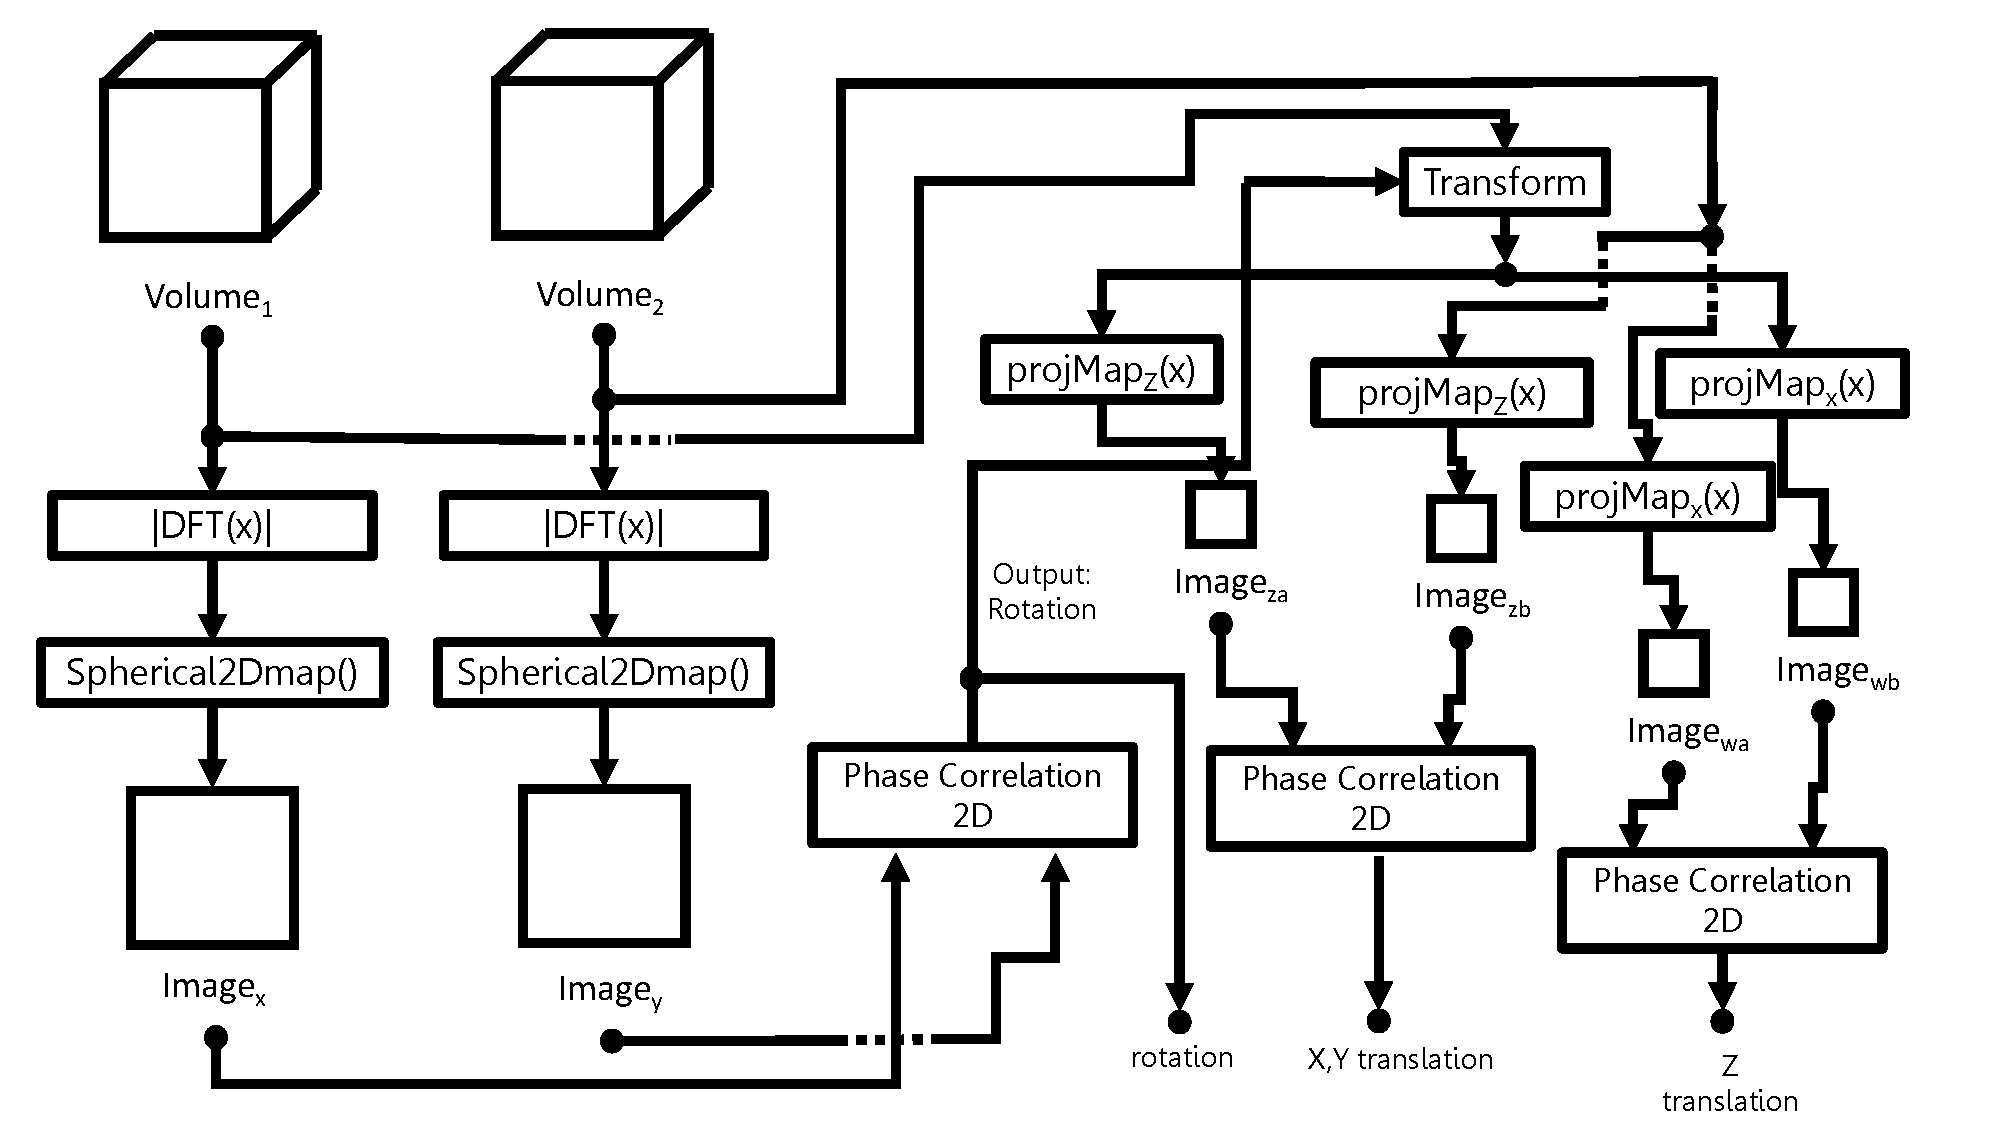
\includegraphics[width=5.0in]{images/ch2/pipeline3}
\caption{System Diagram for Fast Volume Registration}
\label{fig:PIPELINE3}
\end{figure}

Next, the first 3D frame, $Volume_1$ is transformed by the computed rotation factor. This leaves only a 3D translation transform separating both inputs $Volume_1$ and $Volume_2$. Two projection map transforms of both $Volume_1$ and $Volume_2$ (equivalent to 4 transforms in total) are then used to efficiently find this translation factor. The first projection map transform is along the z-axis. The z-axis projection map transform of $Volume_1$ produces 2D image, $Image_{za}$ the z-axis projection map transform of $Volume_2$ produces 2D image, $Image_{zb}$. Both $Image_{za}$ and $Image_{zb}$ may be phase correlated producing the x and y axis components of the translation separating $Volume_1$ and $Volume_2$. \\

The other two projection map transforms are along the x-axis. The projection map transform of $Volume_1$ produces $Image_{wa}$, whilst the projection map transform of $Volume_2$ produces $Image_{wb}$. These two images ($Image_{wa}$ and $Image_{wb}$) may be phase correlated producing the z-axis component of the translation. A composite registration matrix aligning $Volume_1$ to $Volume_2$ may be formed by translating each volume's center to the origin, rotating by the computed rotation factor, translating the origin to the volume's center and finally translating by the $[X,Y,Z]^T$ translation vector computed. \\

Noticeably, the Hanning window function and post $|DFT|(x)$ $Log(x)$ function from the original pipeline (figure \ref{fig:PIPELINENo1}) are missing. The Hanning window function may be incorporated in the first phase correlation procedure, which processes 2D images, therefore the Hanning window function would be in 2D rather than 3D which also improves efficiency as an entire dimension is removed from the process. The log function may also be performed as part of the phase correlation procedure, however it was found that the FFVR procedure estimates rotation more reliably using the spherical-transform if the log function is not performed. This saves additional computational power. \\

It is advantageous to use 2D phase correlation over 3D phase correlation from a computational complexity perspective. The 3D Fourier transform has complexity of $N^3 \times Log(N^3)$ whilst the 2D has complexity $N^2 \times Log(N^2)$. Essentially the amount of data to process has been reduced by an entire dimension. The Phase Correlation method requires 2 $\times$ FFTs, 2 $\times$ element-wise computations and 1 $\times$ inverse FFT. The corresponding 3D phase correlation complexity equates to $3N^3Log(N^3) + 2N^3$ whilst the 2D equivalent is only $3N^2Log(N^2) + 2N^2$. \\ 

\subsubsection{Spherical-map transform}
\label{SMTransform}

As noted, the Spherical-Map transform both reduces the 3D volume to a 2D image whilst retaining information about y-axis rotation. In the new domain, and rotation about the y-axis becomes x-axis translation within the output image. The transform requires a single iteration over the input volume, so it has identical complexity to the 3D Log-Polar transform whilst additionally reducing computational complexity further down the pipeline by compacting the data to process from three dimensions to two dimensions.  \\

An example of an input model (figure \ref{fig:bunnyOrigAA}) and the Spherical-Map domain of the model (figure \ref{fig:bunnySPTed}) is shown in figure \ref{fig:smtExample}. The relationship between the input 3D volume $Vol$ and the output 2D image $Im$ is defined using equations \ref{eqn:invLPFuncs}, \ref{eqn:invLPVVF} and \ref{eqn:smtUpdate}. The value of pixel $Im_{x,y}$ located at coordinate $x,y$ is computed by summing the values along a given ray within the volume. The ray is defined by the vector valued function $Ray(x,y,r)$ found in equation \ref{eqn:invLPVVF}. This function takes the x and y coordinates within the image as well as a radius value (the index from the summation in equation \ref{eqn:smtUpdate}) and returns a vector. The vector is used to index the volume and allows the output pixel to include all the values along the ray. \\

\begin{figure}[!htb]
        \centering
        \begin{subfigure}[b]{2.5in}
                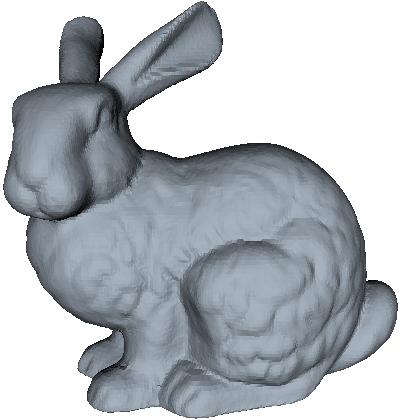
\includegraphics[width=2.5in]{images/ch2/bunny}
                \caption{original}
                \label{fig:bunnyOrigAA}
        \end{subfigure}
        \begin{subfigure}[b]{2.5in}
                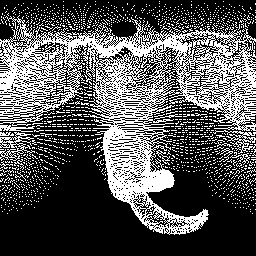
\includegraphics[width=2.5in]{images/ch2/spherical2DMap}
                \caption{transform}
                \label{fig:bunnySPTed}
        \end{subfigure}%
        \caption{The Spherical Map Transform.}
       \label{fig:smtExample}
\end{figure}


Equation \ref{eqn:invLPVVF} is a vector valued function with three separate functions for the x, y and z axis components. These functions are found in equation \ref{eqn:invLPFuncs}. The x-axis function $Ray_x(x,y,r)$ is used together with the $Ray_y(x,y,r)$ and $Ray_z(x,y,r)$ functions to form a spherical transform. The reduction in dimension is achieved by summing the components which share x and y coordinates but have different $r$ (radius) values. In these equations the 3D volume $Vol$ has a width, height and depth of $N$ whilst the output image $Im$ has a width and height of $M$. \\


\begin{equation} \label{eqn:invLPFuncs}
\begin{split}
Ray_x(x,y,r) & = r \times cos\left(\frac{360x}{M}\right)sin\left(\frac{180y}{M}\right)  + \frac{N}{2} \\
Ray_y(x,y,r) & = r \times cos\left(\frac{180y}{M}\right) + \frac{N}{2} \\
Ray_z(x,y,r) & = r \times sin\left(\frac{360x}{M}\right)sin\left(\frac{180y}{M}\right) + \frac{N}{2}
\end{split}
\end{equation}

\begin{equation} \label{eqn:invLPVVF}
Ray(x,y,r) = [Ray_x(x,y,r), Ray_y(x,y,r), Ray_z(x,y,r)]^T
\end{equation}

\begin{equation} \label{eqn:smtUpdate}
Im_{x,y} = \sum_{r=1}^{(2^{-1}N)^{1.5}}{Vol(Ray(x,y,r))} 
\end{equation}

In the Log-Spherical transform described in section \ref{Sec:RoteZoomingSection} re-arranges the rotation and scale transforms along two axis, the third axis retains information and increases the accuracy of the solution. By reducing the other axis from size $N$ to the average value (size 1) information is lost, however computational complexity is reduced by an entire dimension. This is a complexity/performance trade off. Computational complexity may be afforded given input data contains relatively little noise. The output image maps 3D y-axis rotation to 2D x-axis translation is the output image. \\


This process essentially sums up the values along a given ray defined by scaling spherical coordinates and adding up the values intersecting the ray. The resulting image, maps 3D y-axis rotation to 2D x-axis translation. Once two 3D frame volumes $V_a$ and $V_b$ are transformed into their corresponding spherical-map domain $SM_a$ and $SM_b$ respectively, the two may be phase correlated  in order to measure the x-axis translation separating them. This x-axis translation may then be mapped directly to the rotational angle separating the two input 3D camera frames.The relationship may be computed as $\frac{360x}{M}$ where $x$ is the a-axis translation and $M$ is the width and height of the spherical map domain image. \\


\subsubsection{Projection-map transform}
\label{sec:PMTramsform}

The projection map transform is similar in spirit to an orthogonal projection of the volume along a particular axis. Instead of simply projecting the closest point as in projection for visualization purposes, the sum of values computed along the ray is used for representation. The projection map transform is described here in terms of an output projection map image $Im$ and an input 3D volume frame $Vol$, which may be input from a sensor or software system which is able to generate 3D frames of the environment. Each pixel in $Im$ has its value defined mathematically as the summation of values along a particular axis given the x,y coordinates. The Projection-map x-axis transform and the Projection-map z-axis transform are defined in equations \ref{eqn:xPMT} and \ref{eqn:zPMT} respectively. \\

WARNING: add in a picture here

\begin{equation} \label{eqn:xPMT}
Im(z,y) = \sum_{x=0}^{N}{Vol(x,y,z)}
\end{equation}

\begin{equation} \label{eqn:zPMT}
Im(x,y) = \sum_{z=0}^{N}{Vol(x,y,z)}
\end{equation}

In these equations the Projection map transform along the x-axis is computed via summing up values along the x-axis in the input 3D frame,. In this was, any 3D z-axis translation in $Vol$ maps to 2D x-axis translation in the output image $Im$. Additionally any y-axis translation in the input 3D frame $Vol$ is mapped to a corresponding y-axis translation in the output 2D Projection map domain $Im$. If both the width and height of the output image $Im$ is equal to the width, height and depth of the input 3D frame then the relationship is a $1:1$ mapping between 3D z-axis translation and 2D x-axis translation as well as 3D y-axis translation to 2D y-axis translation. \\

The corresponding z-axis Projection map transform sums up values along the z-axis. Here, 3D y-axis translations within the original 3D frame also produce 2D y-axis translations in the output Projection map domain. However, all x-axis translations occurring within the 3D frame domain are mapped to 2D x-axis translations in the output Projection map domain image $Im$. \\

Given both of these Projection map transforms, the 3D translation separating two 3D frames may be registered with respect to 3D translation. This 3D translation also has an inverse relationship to the camera location separation between the two frames. Both 3D frames are transformed into the z-axis Projection map domain. By phase correlating these domains, both the x and y axis translation may be retrieved which map directly to the 3D translation x and y coodinates separating the input frames. The 3D z-axis translation may be computed by transforming both frames into the x-axis Projection map domain. Once the two Projection map domains are phase correlated, the x-axis translation separating the domains can be mapped directly to the corresponding z-axis translation separating the two input 3D frames. In total, using $2 \times$ Projection map transforms and $1 \times$ 2D phase correlation method, the 3D translation parameters separating two 3D frames may be computed. \\

\subsubsection{Performance Analysis}

In order to assess the efficiency gain between the Fast Fourier Volume Registration method over the original FVR method, the computational complexity of the FVR is assessed. The computational complexity is dependent on two factors: the size of the input depth map $W \times H$ and the width/height/depth of the 3D volumes used in the volume registration procedure. Since the computational complexity is fixed no matter the input data (depending only on the sizes specified by the user), this method is considered a closed form solution. \\

The FVR method makes use of several sub-procedures including: projection of the depth frame to a 3D volume frame, 2 $\times$ Hanning window filters, 2 $\times$ 3D FFTs, 2 $\times$ element-wise Log filters, 2 $\times$ Log-spherical transforms, 2 $\times$ 3D phase correlation processes, 1 $\times$ linear transformation and 1 $\times$ peak search. The number of operations required by each of these methods are listed in table \ref{table:complexities} \\

%translation
\begin{table}[ht]
\centering
\scalebox{0.75}{
\begin{tabular}{cc}
\hline
\textbf{Procedure} & \textbf{Complexity}\\ \hline
Hanning window & 26 (GPGPU)\\
3D FFT & $N^3\log{N^3}$ (GPGPU)\\
Log & 3 (GPGPU) \\
Log-Spherical & 58 (GPGPU)\\
Multiplying Spectra & 15 (GPGPU)\\
Geometric Transform & 30 (GPGPU)\\
Peak Search & $2N^3$\\
\\
\end{tabular}}
\\
\caption{Complexities for given Procedures}
\label{table:complexities}
\end{table}[ht]

The Hanning windowing function requires 26 operations. The 3D FFT has complexity of $3N^3\log{N}$, the log and log-spherical transform functions require 3 and 58 operations per voxel respectively. Multiplying two frequency spectra together and transforming a volume requires 15 and 30 operations per voxel respectively. Finding the peak value requires $2N^3$ operations. The complexity in terms of number of operations for the phase correlation process is given in Eq. \ref{eqn:PCFULLPERFORMANCE} This process requires 2 $\times$ 3D FFTs, 1 $\times$ frequency spectra multiplication, and 1 $\times$ peak finding operation. 
\begin{equation} \label{eqn:PCFULLPERFORMANCE}
6N^3\log{N} + 2N^3 + 15
\end{equation}
The total complexity can then be found by taking into account the projection and re-sampling totals as well as the total for $VolumeRegister{\theta \varphi t_x t_y t_z}(V_1, V_2)$. Tallying the number of operations for each process and multiplying them by number of times the process is performed gives us the number of operations as a function of $W$, $H$ and $N$ in Eq. \ref{eqn:FULLPERFORMANCE}.
\begin{equation} \label{eqn:FULLPERFORMANCE}
6N^3 + 28WH + 18(N^3\log{N}) + 230
\end{equation}

To compare performance of the generic volume registration method with the speed up, we use the complexity defined in equation \ref{eqn:FULLPERFORMANCE}. Here, we ignore the cost of projecting the depth map. The 3D DFT has complexity $3N^3log(N)$. This is the first step (see figure \ref{fig:PIPELINE3}), the next is the spherical-map transform which is complexity $45N^3$. If processed on the GPU the performance becomes 45 operations per voxel assuming that one voxel is assigned to one unit of processing. A 3D transform is 30 operations per voxel, 2D phase correlation requires 15 operations to multiply the frequency spectra and $2N^2log(N)$ operations to do the 2D FFT. Finally a projection map transform requires 1 operation per voxel. \\

In total, the proposed method requires $2 \times$ 3D FFTs, $2 \times$ spherical-map transforms, $1 \times$ 3D geometrical transformation, $3 \times$ 2D phase correlations and $4 \times$ projection map transforms. The total complexity is added up for all of these functions and given in equation \ref{eqn:FULLPERF2}. \\

\begin{equation} \label{eqn:FULLPERF2}
6log(N)\times (N^3 + N^2) + 169
\end{equation}

Figure \ref{fig:perfComp} provides a visualization of the performance improvement which the proposed method achieves over the original Fourier volume registration approach. It is clear that the proposed method is around 3 times faster
than the original Fourier based volume registration approach. This is due to the reduction in the amount of data to process afforded by the novel spherical-map transform and orthogonal projection methods.

\begin{figure}[!htb]
\centering
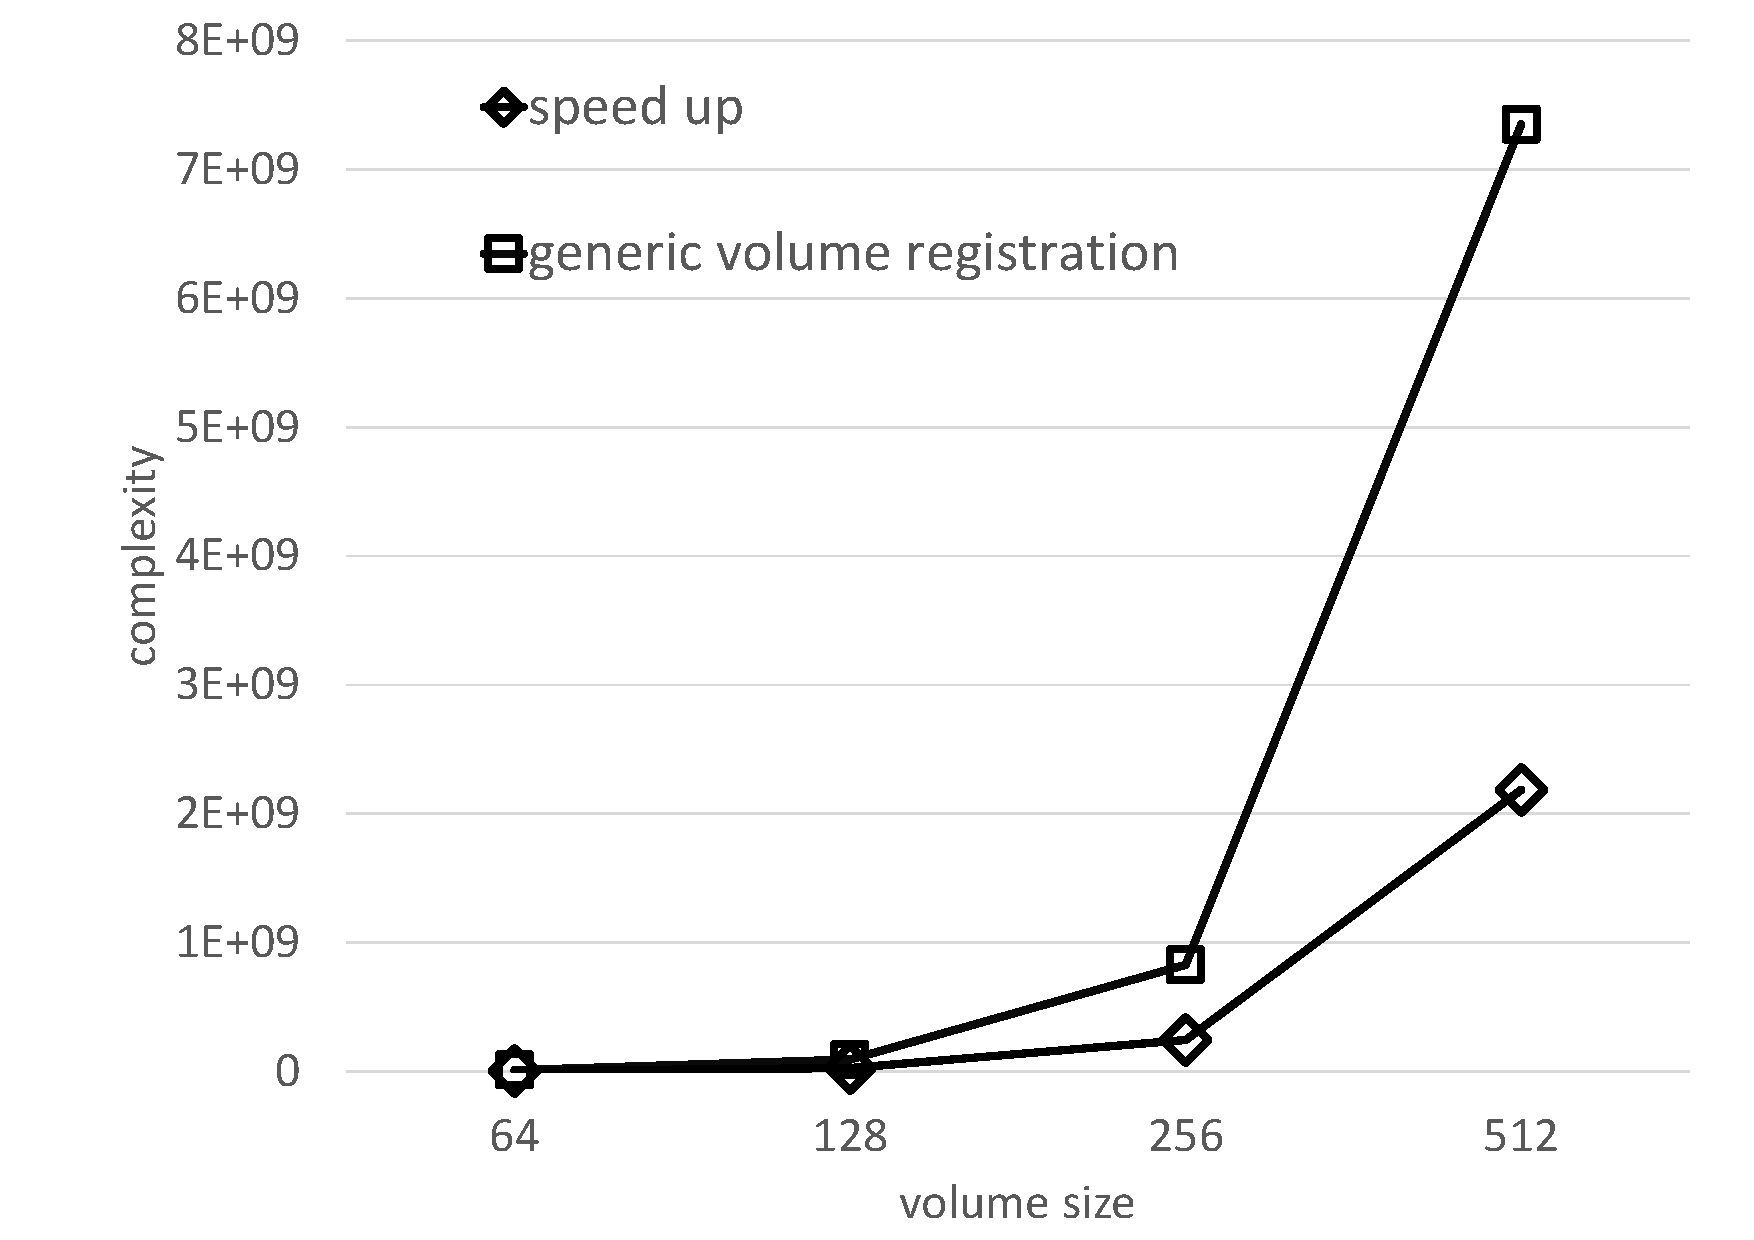
\includegraphics[width=4.0in]{images/ch2/perfcomp}
\caption{Comparison of performance between volume registration and the proposed speed up for different volume sizes.}
\label{fig:perfComp}
\end{figure}

\subsection{Full 3D Rotation Recovery and Reconstruction}

This section explains how the FVR algorithm may be extended to recover full 3D camera pose rotation in addition to translation and scale differences between a pair of captured 3D frames. We propose a novel method which uses Principal Components Analysis (PCA) as a pre-processing step to achieve full 3D rotation estimation. This method is named FVR-3D. The FVR method, the FFVR method and the FVR-3D method all have unique advantages and disadvantages. FVR is designed to be an accurate and efficient method of estimating camera pose and location on wider baselines whilst remaining robust to the effects of noise. It is robust to 3D rotations (not just y-axis rotation) but cannot register them, if 3D rotation recovery is required, the FVR-3D method discussed in this section provides an efficient solution, but is less robust to noise and wider baselines. The FFVR method may also be used, it works similarly to the FVR method but is computationally more efficient at the expense of accuracy and noise robustness. FFVR also cannot handle wide baselines well, but is up to 4 times more efficient than the FVR for realistic volume sizes. \\

To integrate 3D rotation into the standard FVR method, a single axis relating the two 3D models must be known. If such an axis is known prior to executing the FVR method, both 3D frames may be aligned vertically (along the y-axis) with respect to the found axis. Once aligned, the FVR method may be used to register both frames relative to the final y-axis rotational separation which can be used to recover rotation and scale factors so translation may also be recovered. \\

Several techniques were explored to compute this commonly rotated axis. These include computing the average normal value, the axis defined as the vector between the furthest two points as well as other techniques based on feature matching. The use of PCA was also tested. Based on empirically driven factors, PCA was chosen to compute the common axis for use in the FVR-3D method. PCA may be used to compute the full rotation separating two 3D frames but this typically fails when noise or non-overlapping parts of the frames are present. To be more robust to noise and non-overlapping features within the frame, only the primary axis is used to align both frames with their primary axes pointing directly up. This alignment is more robust because the primary axis has a stronger presence within the data. Once the y-axis rotation is solved, the full 3D rotation factors may be computed via the FVR method. \\

Experiments evaluating FVR-3D in section \ref{Sec:FVRSOTA} show it outperforms other popular methods used for 3D camera pose estimation in terms of accuracy on a wide range of scene types. Additional experiments prove its robustness in the face of noise when registering camera pose. \\

\subsubsection{Computing a Principal Axis}

Using PCA to compute the principal axis used in FVR-3D is discussed in this section. Both 3D frames have their axis computed separately before they are used to align both frames to a common axis. To compute the common axis using PCA, both the eigen-values and eigen-vectors of the covariance matrix of the 3D frames must be computed. The eigen-vector with the largest corresponding eigen-value is set as the primary axis. The procedure works as follows. \\

Given a 3D point cloud $A$ of $N$ points, which may be generated via monocular methods, stereo disparity estimation or active sensor (Kinect, Asus XTion Pro-LIVE), the co-variance of the points between two of the dimensions ($x$ and $y$) is computed as the summation of each $x$ component subtracted by the mean $x$ value multiplied by the $y$ component subtracted by the mean $y$ component value (see equation \ref{eqn:Covariance3DSignal}, $A_{x_{mean}}$ and $A_{y_{mean}}$ refer to the mean values of these x and y dimensions of $A$). \\

\begin{equation} \label{eqn:Covariance3DSignal}
Cov(A_x,A_y) = \sum_{i=0}^{N}(A_{x_i} - A_{x_{mean}})(A_{y_i} - A_{y_{mean}})
\end{equation}

Using the formula for covariance the covariance matrix may be computed for an $N$ dimensional signal. In the case of 3D construction, this matrix is a $3 \times 3$ covariance matrix where each column/row index represents a covariance relationship. This covariance matrix is shown in equation \ref{eqn:CovarMatrix}. This matrix describes how each coordinate axis changes with respect to each other coordinate. The eigen-vectors of this matrix constitute the principal components of the 3D point cloud frame. \\

\begin{equation} \label{eqn:CovarMatrix}
\left[
\begin{array}{ccc}
Cov(A_x, B_x) & Cov(A_x, A_y) & Cov(A_x, A_z) \\
Cov(A_y, B_x) & Cov(A_y, A_y) & Cov(A_y, A_z) \\
Cov(A_z, B_x) & Cov(A_z, A_y) & Cov(A_z, A_z) \\
\end{array}
\right]
\end{equation}

The three eigen-vectors of the covariance matrix describe the primary axis of the 3D frame $A$ and the three corresponding eigen-values describe the dominance of these vectors. The eigen-vector/axis with the largest corresponding eigen-value is the principal component in PCA and is used as the aligning axis in the FVR-3D method. This principal axis is used to align data to a common axis defined as the vertical y-axis. For simplicity, the principal axis of a 3D frame $A$ is written as $A_{pa}$. During the PCA process, the centroid of the point cloud is also computed. This is simply the average point location within the input point cloud. For simplicity in later discussions, the centroid of a 3D frame $A$ is written as $A_{mean_{location}}$. A visualization of the principal axis and centroid are shown in Figure \ref{fig:FVR3D111}. Here two input frames (Figures \ref{fig:fvr3DINA} and \ref{fig:fvr3DINB}) are corrected such that their mean is translated to the centre of the volume and their principal axis is aligned with the vertical axis (Figures \ref{fig:fvr3DAAlign} and \ref{fig:fvr3DBAlign}). \\

\begin{figure}[!htb] 
        \centering
        \begin{subfigure}[b]{3.0in}
               \centering
                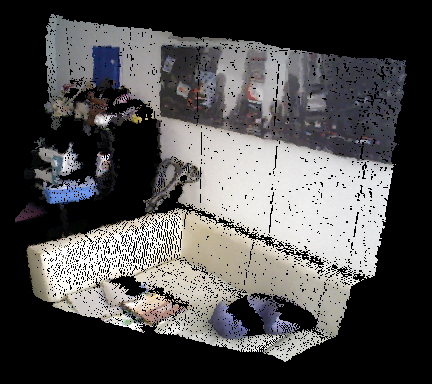
\includegraphics[width=2.0in]{images/methodology/FVR/fvr3d/frameA}
                \caption{Frame A}
                \label{fig:fvr3DINA}
        \end{subfigure}%
        \begin{subfigure}[b]{3.0in}
        		\centering
                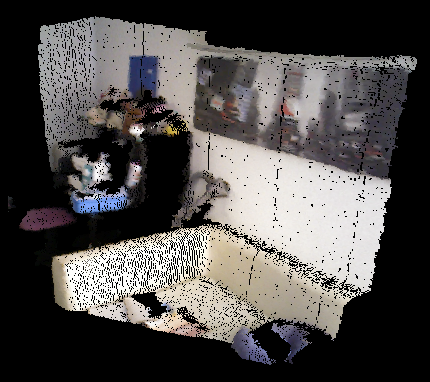
\includegraphics[width=2.0in]{images/methodology/FVR/fvr3d/frameB}
                \caption{Frame B}
                \label{fig:fvr3DINB}
        \end{subfigure}
        
         \begin{subfigure}[b]{3.0in}
         		       \centering
                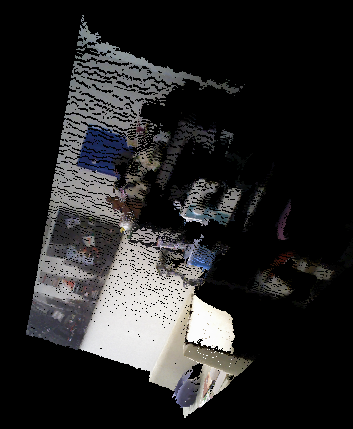
\includegraphics[width=2.0in]{images/methodology/FVR/fvr3d/PCAFrameA}
                \caption{Frame A, PCA aligned}
                \label{fig:fvr3DAAlign}
        \end{subfigure}%
         \begin{subfigure}[b]{3.0in}
                \centering
                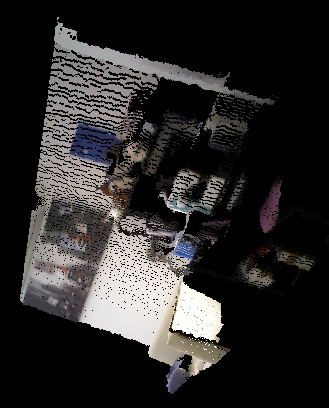
\includegraphics[width=2.0in]{images/methodology/FVR/fvr3d/PCAFrameB}
				\caption{Frame B, PCA aligned}
                \label{fig:fvr3DBAlign}
        \end{subfigure}
        

       \caption{Early stages of FVR-3D}
       \label{fig:FVR3D111}
\end{figure}



\subsubsection{Alignment Pre-Process}

Using the PCA method, for each input 3D frame $V$, the computed principal axis $V_{pa}$ and the centroid $V_{mean_location}$ are used to align the input 3D frame using $V_{pa}$ as the new vertical axis. To this end, a transformation matrix is formed and used to rotate the volume so the principal axis $V_{pa}$ points up. This is useful because if a 3D frame pair are both rotated with respect to their principal axis, and both frames share enough overlap, then only 3D y-axis rotation, 3D translation (and possibly 3D scale) separate the two frames. As discussed in section \ref{Sec:AFVRApproach}, these parameters may be recovered using the FVR method. The matrix used to normalize the 3D frames in terms of their principal axis is discussed here. \\

If $V_{pa}$ (the vector pointing along the principal axis of $V$) is to be set as the new y-axis for the volume, then the other axes must also be computed (x-axis and z-axis). The z-axis, named the forward ($Fwd$) axis, is computed based on the cross product between the then x-axis and the principal axis $V_{pa}$ (taken as the y-axis) which gives a psuedo z-axis. The cross product between the principal axis and this pseudo z-axis gives an accurate x-axis. Lastly the cross product between this x-axis and the y-axis (the principal axis) gives the corresponding z-axis in the form of the variable $Fwd$. This is shown in equation \ref{eqn:fwdVector}. \\


\begin{equation} \label{eqn:fwdVector}
Fwd = \left(\left[
\begin{array}{c}
V_{pa_{x}}\\
V_{pa_{y}}\\
V_{pa_{z}}\\
\end{array}
\right] \times \left(\left[
\begin{array}{c}
1\\
0\\
0\\
\end{array}
\right] \times \left[
\begin{array}{c}
V_{pa_{x}}\\
V_{pa_{y}}\\
V_{pa_{z}}\\
\end{array}
\right]\right)\right) \times \left[
\begin{array}{c}
V_{pa_{x}}\\
V_{pa_{y}}\\
V_{pa_{z}}\\
\end{array}
\right]
\end{equation}

The final axis completing the new space is the x-axis defined at the cross product between the principal axis (the new y-axis) and the z-axis (the $Fwd$ vector) and is named $Rgt$ (standing for right facing axis). Equation \ref{eqn:rgtVector} shows this calculation. The new space is now defined by x-axis $Rgt$, y-axis $V_{pa}$ and z-axis $Fwd$. A rotation matrix transforming original space to the new space defined by these axes may be computed using the $Rgt$, $V_{pa}$ and $Fwd$ axes as the column vectors of the rotation matrix. The inverse, that is the transformation from the new space to the original space may be computed using the transpose of the rotation matrix. The rotation of the point cloud from the new space defined by the principal axis to the original space is useful as it aligns the principal axis to the y-axis leaving only 3D y-axis rotation, 3D translation and possibly scale to be registered. \\ 


\begin{equation} \label{eqn:rgtVector}
Rgt = \left[
\begin{array}{c}
V_{pa_{x}}\\
V_{pa_{y}}\\
V_{pa_{z}}\\
\end{array}
\right] \times \left[
\begin{array}{c}
Fwd_x\\
Fwd_y\\
Fwd_z\\
\end{array}
\right]
\end{equation}

The input 3D frame $V$ may be aligned by its principal axis as the new y-axis by first transforming the centroid to the origin. Next the 3D frame may be rotated from the new space to the default identity space. This sets $Rgt$ as the new x-axis, $V_{pa}$ as the new y-axis and $Fwd$ as the new z-axis. The rotation matrix may be computed as the row vectors of these axes. Finally, after rotation the 3D frame $V$ may be transformed back to the centroid. This aligns the 3D frame so that $V_{pa}$ points towards the y-axis. The compounded transformation to perform this alignment is fully defined in equation \ref{eqn:CorrectUpMat}. \\

\begin{equation} \label{eqn:CorrectUpMat}
CorrectMat(V) = \left[
\begin{array}{cccc}
1 & 0 & 0 & V_{mean_x} \\
0 & 1 & 0 & V_{mean_y} \\
0 & 0 & 1 & V_{mean_z} \\
0 & 0 & 0 & 1 \\
\end{array}
\right] \left[
\begin{array}{cccc}
Rgt_x & Rgt_y & Rgt_z & 0 \\
V_{pa_x} & V_{pa_y} & V_{pa_z} & 0 \\
Fwd_x & Fwd_y & Fwd_z & 0 \\
0 & 0 & 0 & 1 \\
\end{array}
\right] \left[
\begin{array}{cccc}
1 & 0 & 0 & -V_{mean_x} \\
0 & 1 & 0 & -V_{mean_y} \\
0 & 0 & 1 & -V_{mean_z} \\
0 & 0 & 0 & 1 \\
\end{array}
\right]
\end{equation}

\subsubsection{3D Rotation Registration}

To recover a matrix for full 3D rotation separating two input 3D frames $A$ and $B$ which have been taken from two different locations (translation separation) with two different poses (3D rotational separation) and possibly projected differently (scale separation), the first step is to align both frames by their principal axis. The alignment matrix for $A$ can be computed as $C_A = CorrectMat(A)$ and the alignment matrix for $B$ may be computed as $C_B = CorrectMat(B)$. Transforming both $A$ and $B$ by their alignment matrix gives two volumes $A_{aligned} = Transform(A, C_A)$ and $B_{aligned} = Transform(B, C_B)$ which are now only separated by 3D y-axis rotation, 3D translation and 3D scaling factors. As discussed in sections \ref{Sec:VolumeRegistrationSection} and \ref{Sec:AFVRApproach} these factors may be computed and a registration matrix aligning $A_{aligned}$ and $B_{aligned}$ generated. This matrix is computed as $R_{y}ST = FVR(A_{aligned},B_{aligned})$. Using this registration matrix and the alignment matrices $C_{A}$ and $C_{B}$, the full 3D registration matrix $R_{x,y,z}ST$, which transforms $A$ to $B$, may be computed. Matrix $R_{x,y,z}ST$ aligns $A$, registers it using $R_{y}ST$ (which aligns it with $B_{aligned}$) then inverse transforms it by $C_{B}$ which un-aligns it according to alignment matrix $C_B$. This can be followed as in equation \ref{eqn:FullRSTTransform}. \\


Figure \ref{fig:FVR3D222} (along with Figure \ref{fig:FVR3D111}) shows the output at different stages of the FVR-3D technique. Once two input frames (Figures \ref{fig:fvr3DINA} and \ref{fig:fvr3DINB}) are aligned via PCA (Figures \ref{fig:fvr3DAAlign} and \ref{fig:fvr3DBAlign}), they must be registered using the FVR method. This is shown in Figure \ref{fig:fvr3DFVRPCAAB}, as without any further registration, the reconstruction would not be correct (see Figure \ref{fig:fvr3DPCAAB}). By reversing Frame B's PCA alignment stage on the frame in Figure \ref{fig:fvr3DFVRPCAAB} the full FVR-3D registration output is revealed (Figure \ref{fig:fvr3DFVRPCAAB}). This registration is very accurate in comparison to zero registration being performed prior to integration, which is shown in Figure \ref{fig:fvr3DPCAAB}. \\
 

\begin{equation} \label{eqn:FullRSTTransform}
R_{x,y,z}ST Matrix = C_{B}^{-1} \times R_{y}ST \times C_A
\end{equation}

FVR-3D is a capable registration method which extends Fourier registration to take into account full 3D rotation. The complexity of the technique adds a single layer of complexity over the FVR method. The additional computational complexity ($N^3$), which is primarily made up of computing the covariance matrix, is minimal compared to the rest of the FVR technique. \\


\begin{figure}[!htb] 
        \centering
        
		\begin{subfigure}[b]{3.0in}
				       \centering
                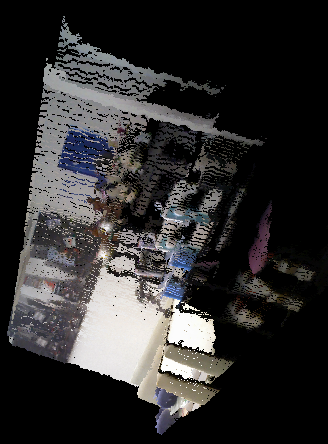
\includegraphics[width=2.0in]{images/methodology/FVR/fvr3d/PCAFrameAB}
                \caption{\ref{fig:fvr3DAAlign} and \ref{fig:fvr3DBAlign} integrated}
                \label{fig:fvr3DPCAAB}
        \end{subfigure}%
        \begin{subfigure}[b]{3.0in}
               \centering
                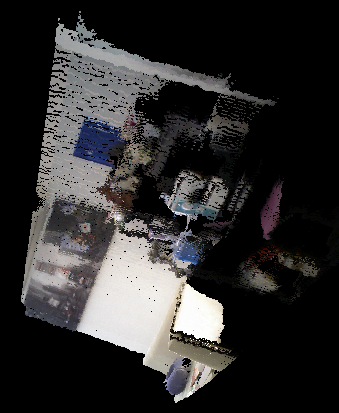
\includegraphics[width=2.0in]{images/methodology/FVR/fvr3d/FVRPCAFrameAB}
                \caption{\ref{fig:fvr3DAAlign} registered with \ref{fig:fvr3DBAlign} using FVR}
                \label{fig:fvr3DFVRPCAAB}
        \end{subfigure}        
        
        \begin{subfigure}[b]{3.0in}
               \centering
                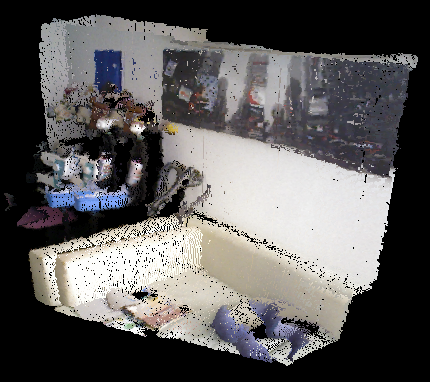
\includegraphics[width=2.0in]{images/methodology/FVR/fvr3d/noRegistration}
                \caption{\ref{fig:fvr3DINA} and \ref{fig:fvr3DINB} integrated}
                \label{fig:fvr3DPCAAB}
        \end{subfigure}%
        \begin{subfigure}[b]{3.0in}
               \centering
                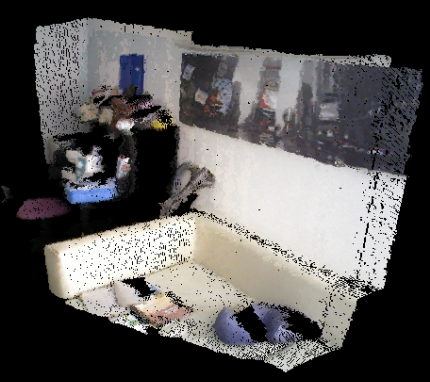
\includegraphics[width=2.0in]{images/methodology/FVR/fvr3d/FVR3DReg}
                \caption{\ref{fig:fvr3DFVRPCAAB} un-aligned (full FVR-3D registration)}
                \label{fig:fvr3DFVRPCAAB}
        \end{subfigure}        
        
       \caption{Final stages of FVR-3D}
       \label{fig:FVR3D222}
\end{figure}



\subsubsection{Algorithm and Pipeline}

\label{METHOD_SECLL}

The proposed SLAM/3D reconstruction routine for the FVR-3D is almost identical to the routine for the FVR method in Listing \ref{algorithm:PCSLAMNo1}. First, the 3D frame $f_1$ is read in and projected to construct a point cloud $PointCloud$. $PointCloud$ is then integrated using volumetric integration into the global reconstruction. Matrix $M$ is initialized to the identity matrix to accumulate the registration matrices so future frames may be efficiently integrated. $Camera_{location}$ and $Camera_{pose}$ accumulate camera location and 3D rotational pose, respectively, and are combined and listed in $Cameras$ on a per frame basis. These variables may be omitted in the case of 3D reconstruction, or output in the case of 3D SLAM. Next, a loop is used for each new frame input into the system. In this loop, 3D frame $f_2$ is read in. Both $f_2$ and $f_1$ are projected and voxelized into $V_1$ and $V_2$, respectively. \\

\begin{figure}
\begin{lstlisting}[language=c++,caption=Phase Correlation Based SLAM Algorithm,label=algorithm:FVR3DSLAM,mathescape,basicstyle=\ttfamily]
$f_1$ = ReadFrame();
$PointCloud$ = project($f_1$);
$GlobalReconstruction$.integrate($PointCloud$)
$M$ = IdentityMatrix();
$Camera_{location}$ = $[0, 0, 0]^T$;
$Camera_{pose}$ = $[[1, 0, 0]^T,[0, 1, 0]^T,[0, 0, 1]^T]$;
$Cameras$ = $\left[\left[Camera_{location}, Camera_{pose}\right] \right]$;
while(more frames){
	$f_2$ = ReadFrame();
	$points_1$ = project($f_2$);
	$points_2$ = project($f_1$);
	$V_1$ = Voxelize($points_1$);
	$V_2$ = Voxelize($points_2$);
	$R_{x,y,z}ST$ = $FVR-3D_{\theta \varphi t_x t_y t_z}(V_1, V_2)$;
	$Temp$ = $R_{x,y,z}ST$;
	$M = M \times Temp$;
	$points_1$ = Transform($points_1$, $M$);
	$GlobalReconstruction$.integrate($points_1$);
	$Camera_{location}$ = $Temp^{-1} \times Camera_{location}$;
	$Camera_{pose}$ = $Temp^{-1} \times (Camera_{pose} + Camera_{location})$;
	$Camera_{pose}$ = $\frac{Camera_{pose} - Camera_{location}}{Camera_{pose} - Camera_{location}}$;
	$Cameras.add(\left[Camera_{location}, Camera_{pose}\right])$;
	$f_1$ = $f_2$;
}
\end{lstlisting}
\end{figure}

Next, the FVR-3D method is used in place of the FVR method to compute the full six (plus 1 for scale) degrees of freedom required for 3D SLAM or 3D reconstruction. A temporary variable $Temp$ is used to hold this rigid transformation matrix. $M$ is then updated to take into account the previous registration transforms plus the current one. Using the updated transformation matrix, $M$ is applied to $points_1$ to register it with the current global reconstruction, then integrated with the final reconstruction. Next, $Camera_{location}$ and $Camera_{pose}$ are updated and the new camera pose and location values are added to the $Cameras list$. \\



Figure \ref{fig:PIPELINE8} shows a pipe-line for the FVR-3D technique. Here, two 3D frames are input as $Volume_1$ and $Volume_2$. The second frame may be taken after the camera has changed location and pose. The two frames may also be taken by different cameras with differing projection procedures projecting depth map values into frames. First the alignment matrices $C_a$ and $C_b$ based on the principal axis are computed by the PCA algorithm. These matrices are then used to align $Volume_1$ and $Volume_2$ to a common axis. Only then can the proposed FVR method be used to register the final axis of rotation along with scale and translation changes. Finally a full registration matrix may be formed by the alignments matrices and the output registration matrix via the FVR procedure. \\

\begin{figure}[!htb]
\centering
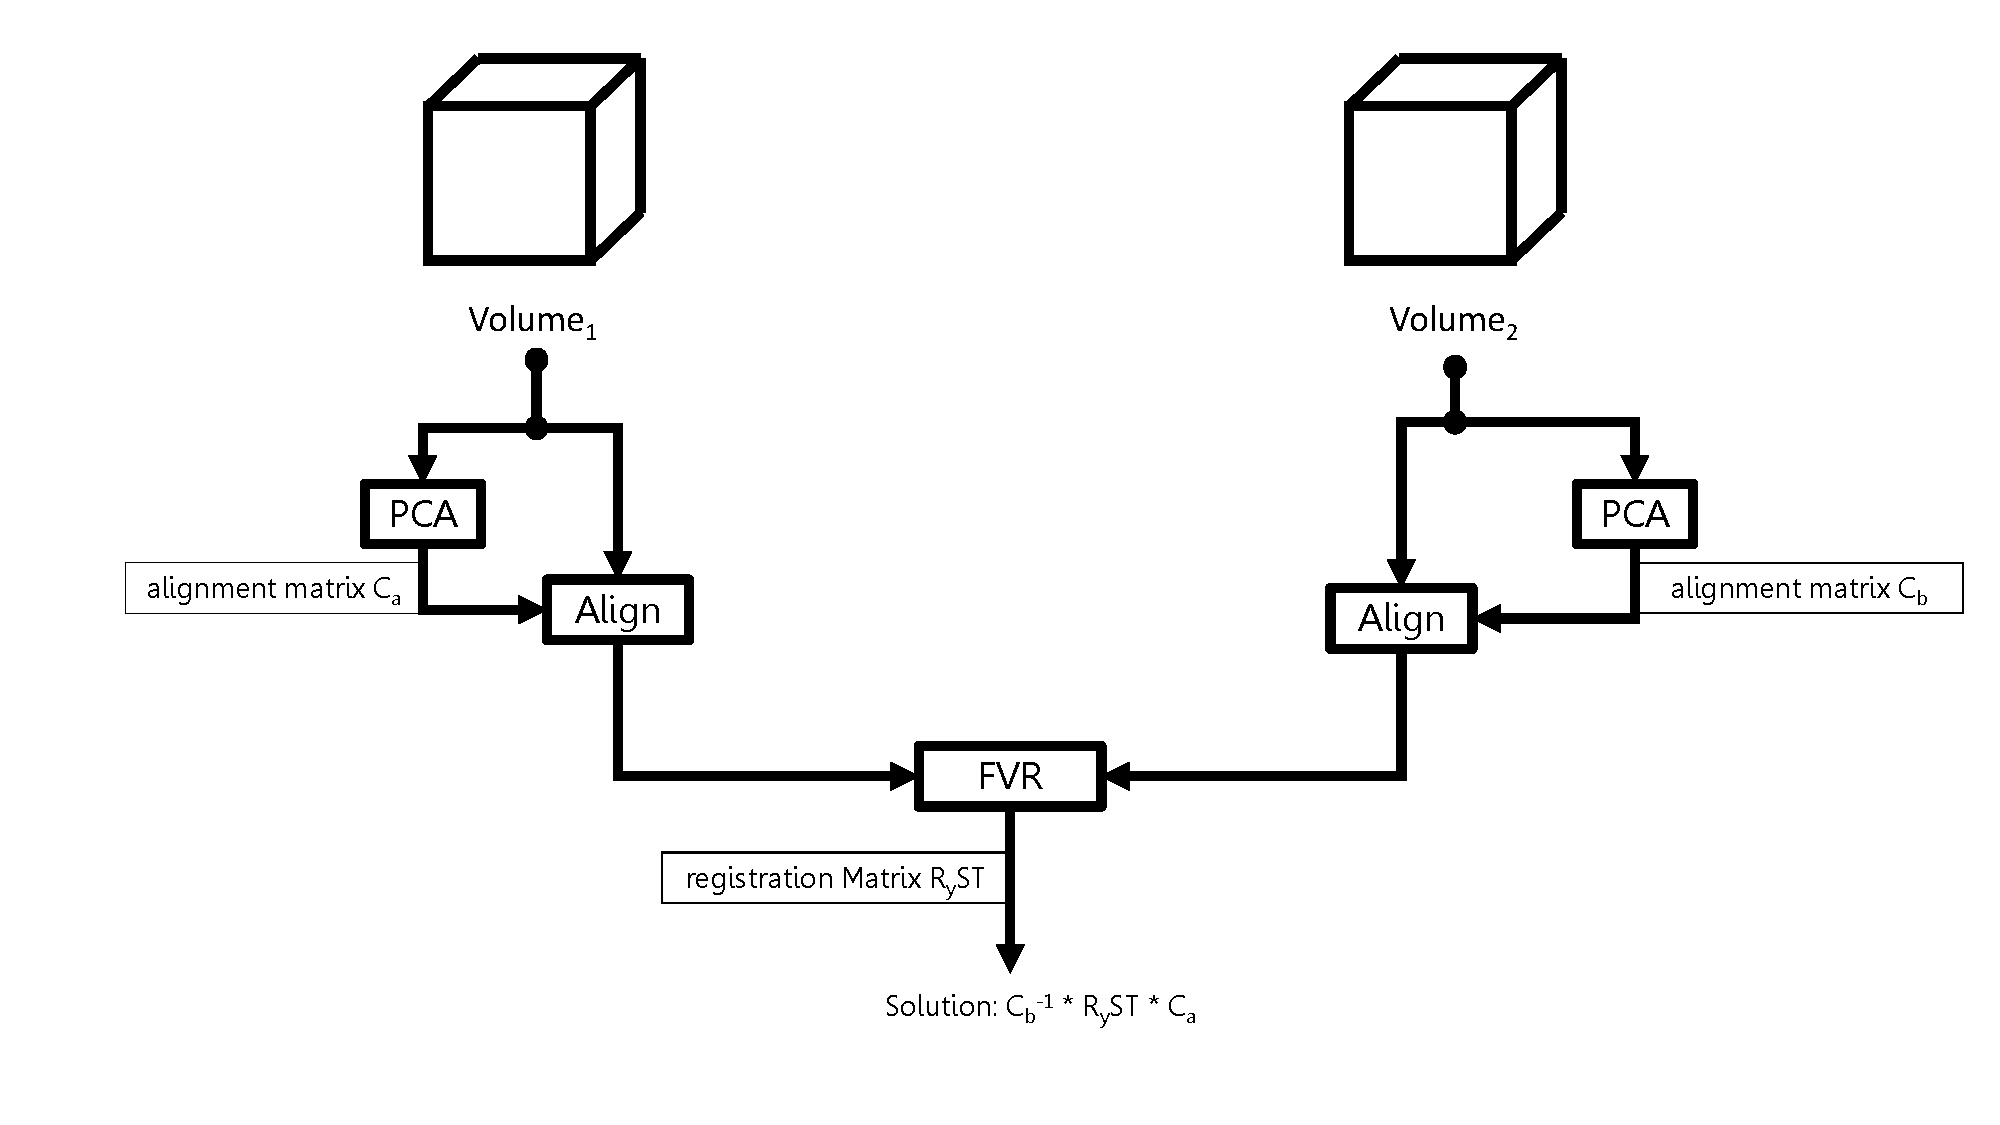
\includegraphics[width=6.0in]{images/methodology/FVR/pipeline8}
\caption{System Diagram for Registration Process}
\label{fig:PIPELINE8}
\end{figure}


\subsubsection{Limitations}

Experiments (sections \ref{Sec:FVRSOTA} and \ref{Sec:CamTransTrackExp}) show that the FVR-3D algorithm is a capable 3D reconstruction method in terms of accuracy, however, it is less robust to noise and wide-baselines than the FVR method. This is due to PCA being much more affected by noise than the FVR method on its own. Therefore, whilst the FVR method is limited to y-axis rotational registration, it is more robust under noisy conditions. To solve this noise issue associated with FVR-3D, the plain FVR method is also used whenever FVR-3D is used and the best registration is chosen on a per frame basis. Despite the reduced accuracy at wide baselines or when more noise is present, the FVR-3D method outperforms several state-of-the-art algorithms used in registering 3D frames produced by different sensor types, including: stereo and active camera set-ups. \\





\section{Plane-Tree Data Compression}
In this section a novel 3D frame data representation and compression method is described. It was designed to help reduce data size whilst facilitating data processing. This novel representation is named Plane-Tree and is a modification of the basic Octree 3D data representation method. \\

The Shade-Tree is designed primarily to compress 3D data. It is based on the Octree but was inspired by the Shade-Tree and Interpolated Leaf Quad-Tree representations \cite{Gonzalez07ShadeTree, Lincoln13Interpolating} which are used for image compression. These techniques make use of Quad-Tree decomposition and have been shown to outperform several transform based methods of compression. 

\subsection{Octree Overview}

In this section Octree decomposition is explained. This strategy forms a cubic shaped space around some 3D data. In the case of 3D reconstruction, it may be the 3D frame input from an active sensor, stereo method or monocular depth estimation procedure. A geometric representation is then computed for the data contained within the cubic space. This representation may be as simplistic as recording the cube's center or using the cube to represent the space, or may be complex, employing splines and curvature representation techniques to represent the space. \\

Whatever the representation, a measurement system must be used to decide whether the computed geometric representation fits the data within the space adequately. If the geometric representation is accurate enough for application purposes, then it may be used in place of the data. This representation is typically designed such that the amount of data required for representation of a space is less than the amount which would be used otherwise. Alternatively, the representation may make use of known correlations which may be more easily compressed compared with the initial representation. \\


\begin{figure}[!htb]
\centering
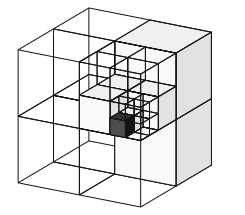
\includegraphics[width=8cm]{images/methodology/pt/octreeVis}
\caption{Visualization of cubic space being split \cite{Hornung13Octomap}.}
\label{fig:SpaceVis}
\end{figure}

If, by the error generated via the measurement system, it is decided the representation is not suitable, the cubic space is broken down into 8 sub-cubes and the process is repeated. For an example of the space broken down into sub-cubes see figure \ref{fig:SpaceVis}. \\

At each level of decomposition, the data representation achieves finer detail, but more nodes must be stored which means less compression. This is a classic trade-off between compression and accuracy in representing the underlying object. An example of the Octree's use in representing an object at differing levels of accuracy is shown in figure \ref{fig:octreeaccuracy}. In the next section, the decomposition procedure is discussed further. Section \ref{sec:dr:coding} describes the geometric representation employed by the Plane-Tree.


\begin{figure}[!htb]
\centering
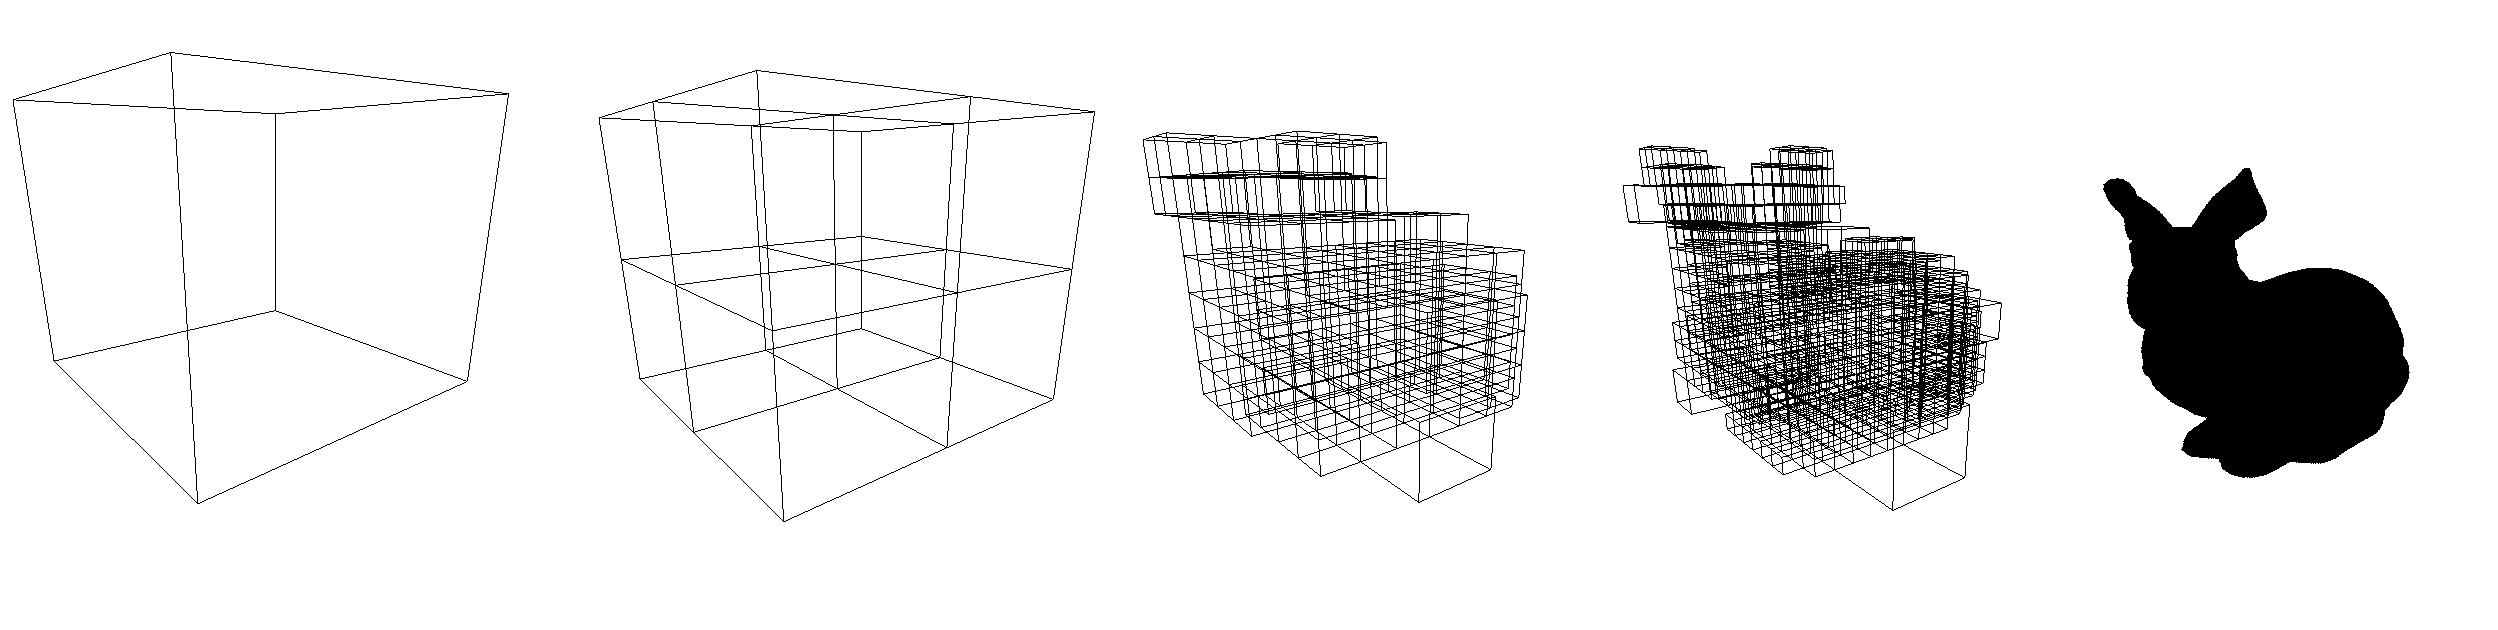
\includegraphics[width=14cm]{images/ch2/OctreeExample}
\caption{An Example of an Octree used to represent an object at differing levels of accuracy \cite{Hornung13Octomap}. Left: Original model, Middle: few node splits used to represent the model. Right: many node splits used to more accurately represent the model.}
\label{fig:octreeaccuracy}
\end{figure}


\subsubsection{Octree Description}
\label{OTDesc}

The Octree is the three dimensional extension to the two dimensional Quad-Tree (QT) technique. First we provide some information about the QT and the idea behind using planes or shading the cubic (or square in the case of the QT) nodes to improve compression and efficiency. This was the fundamental idea behind the Shade-Tree and ILQT algorithms \cite{Gonzalez07ShadeTree, Lincoln13Interpolating}. Both these techniques have been shown to improve compression in comparison to state of the art transforms and form the basis of reasoning behind the Plane-Tree. \\

The QT is a hierarchical data structure used for processing and compressing 2D data. Figure \ref{QuadtreeExample} shows an example of a QT used to represent an image. In this figure, the original image is on the left. The QT first uses a single coloured square to represent the entire image, then using some error metric it decides whether or not to, a) represent the image more accurately using more memory or b) stop decomposition and represent the image with a single colour. If option b) is chosen, the image will look like the second left picture. If option a) is chosen, the image is divided into four sub-images each with its own colour. From here the whole process begins again, with each sub-image given the same options. The final product of the QT is shown on the far right in figure \ref{QuadtreeExample} and a visualization of a QT hierarchy is shown in figure \ref{QuadTreeHierarchy}. \\


\begin{figure}[!htb]
\centering
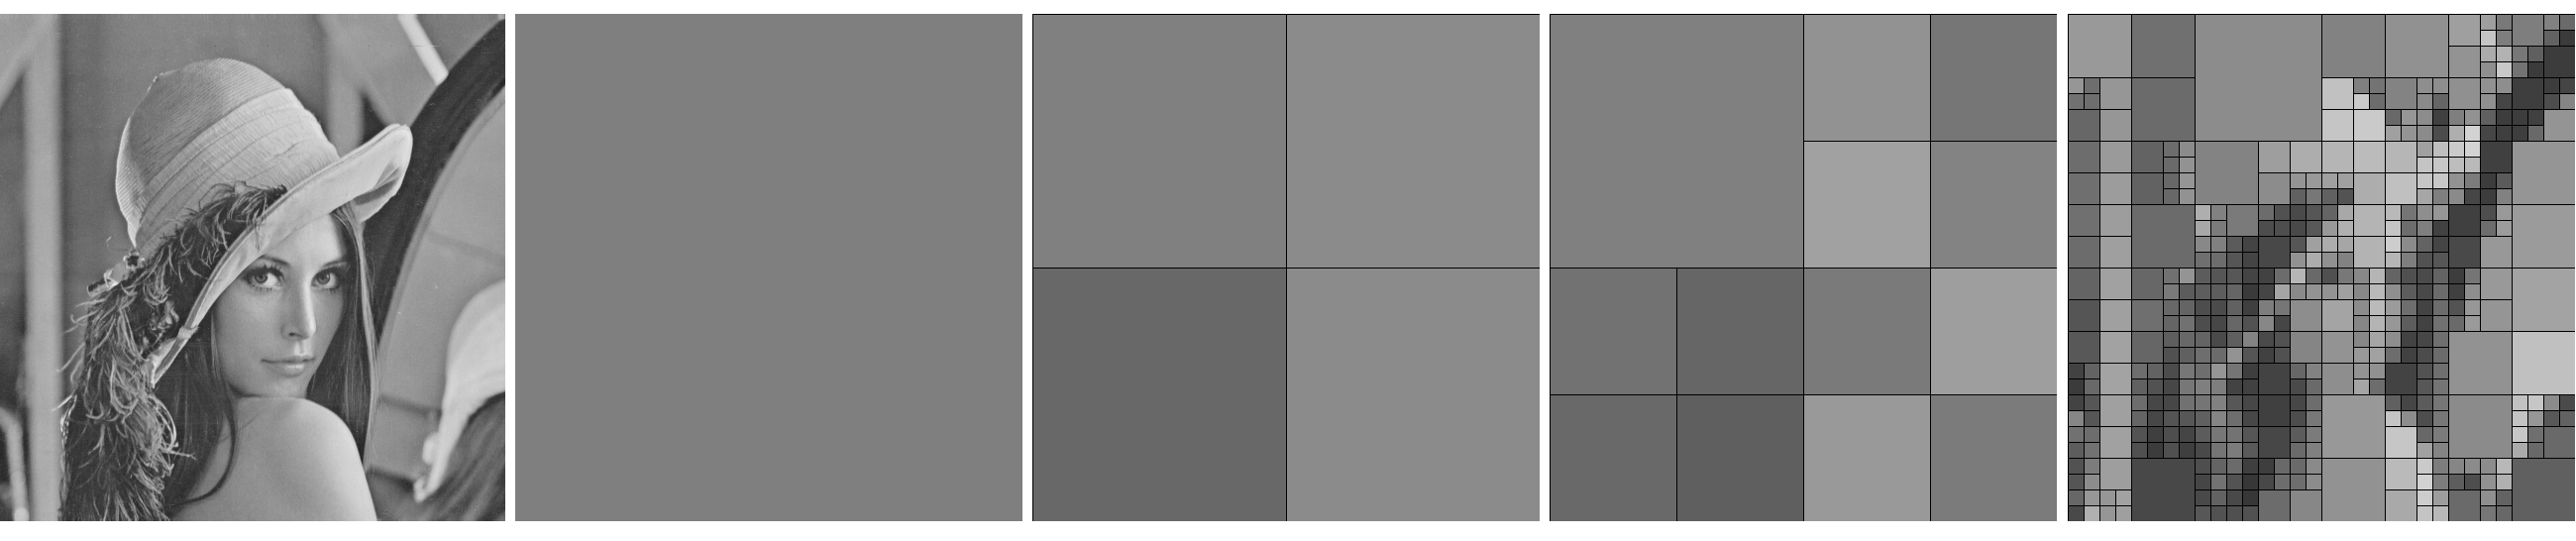
\includegraphics[width=12cm]{images/ch2/quadtreeexample}
\caption{Quadtree Image Representation, left to right: Original Image, 1st Level of Decomposition, 2nd Level of Decomposition, 3rd Level of Decomposition, QT codec Image.}
\label{QuadtreeExample}
\end{figure}


\begin{figure}[!htb]
\centering
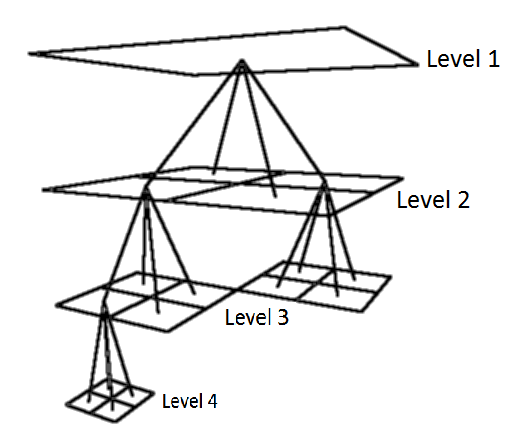
\includegraphics[width=6cm]{images/ch2/QuadTreeHierarchy}
\caption{A visualization of the QT hierarchy}
\label{QuadTreeHierarchy}
\end{figure}

The ILQT and Shade-Tree use small amounts of memory at the corners of the quadrants and interpolate to generate the underlying structure. The small data structures used for representation are much more compressed in their representation compared to the raw pixel data. For this reason, the ILQT and Shade-Tree do not need to decompose as much as other representations and allow for greater compression as proven by their ability to compete with transform based methods. \\

As mentioned, the OT works identically to the QT but in 3D. Instead of surrounding the 2D image with a square encompassing the entire frame, a cube is used to enclose the 3D space. Similarly to the QT, an error metric is used to decide whether the current representation is adequate enough or not. If the octant must be split, it is divided into eight sub-octants. Each split operation divides each coordinate ($x,y,z$) by two, giving the 8 sub-octant spaces. Figure \ref{OctreeExample} shows and example of this decomposition process. The further each cube is split, the more the OT resembles the model being compressed. In the QT and OT, nodes which have not been split are called leaf nodes and the function which decides whether a node should be split is called a leaf criterion function. \\ 

\begin{figure}[!htb]
\centering
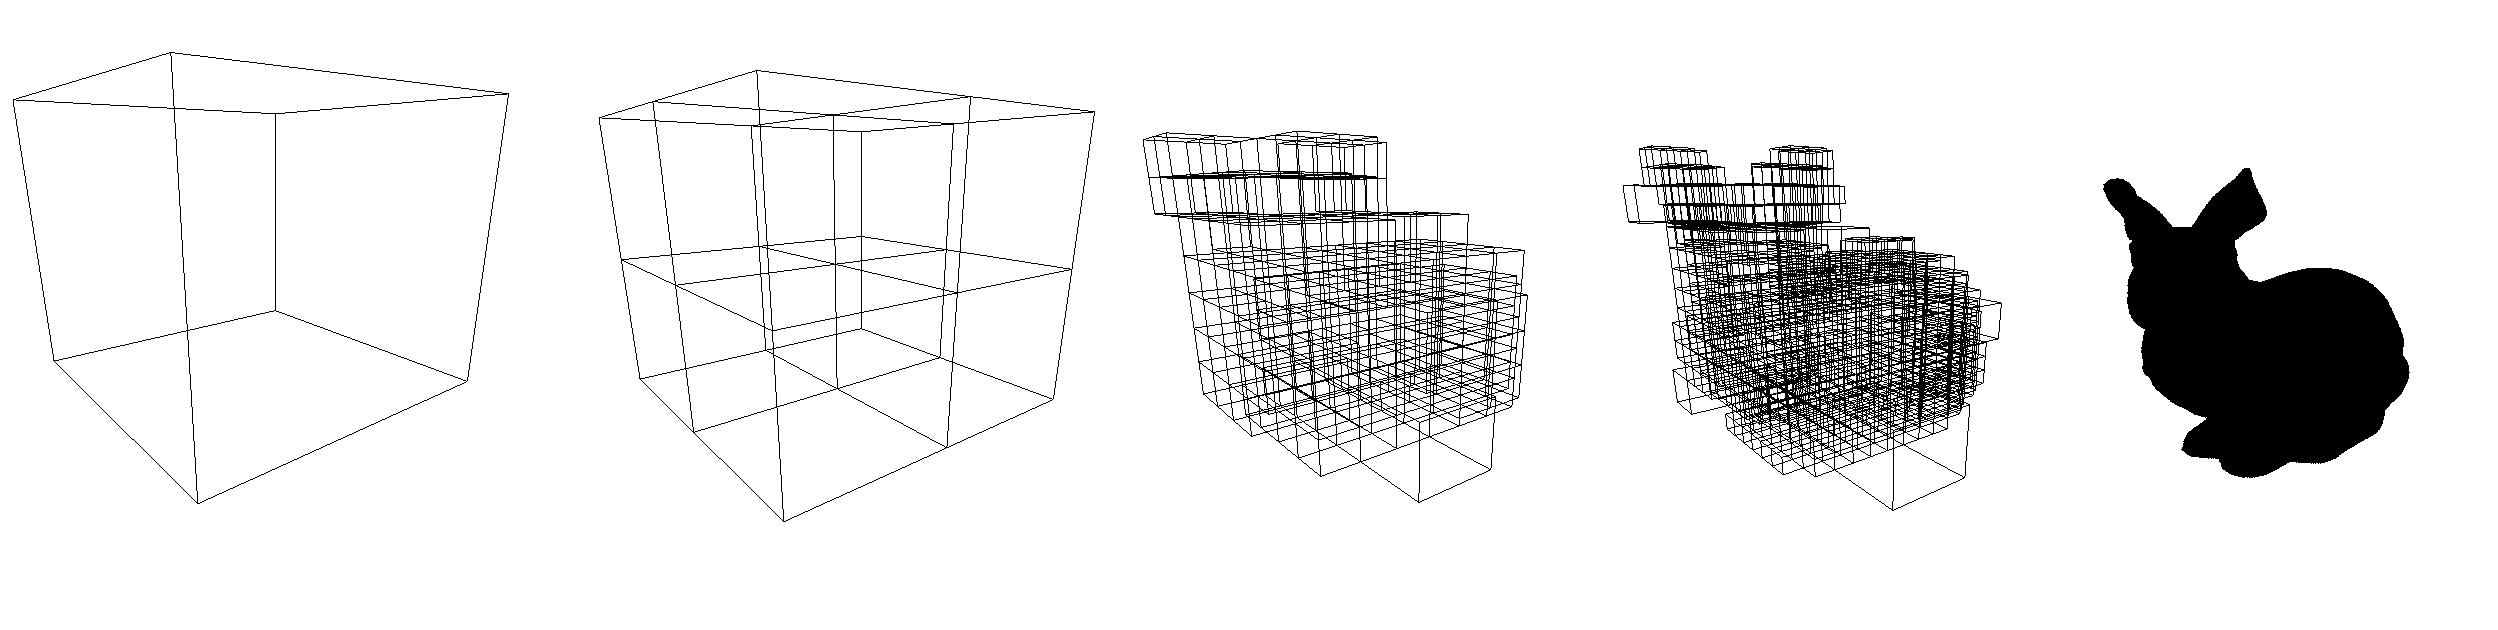
\includegraphics[width=16cm]{images/ch2/OctreeExample}
\caption{Visualization of OT Decomposition}
\label{OctreeExample}
\end{figure}

The goal of the OT and the QT is to store the size and attributes of each node implicitly. There are two main methods of representation, a packed traversal of the tree and a linear tree. The packed traversal method stores the hierarchy using a pre-defined traversal of the tree, and typically follows one of two orderings. These are, breadth-first traversal and depth-first traversal, these orderings are shown in figure \ref{TreeTraversalExample}. The depth-first traversal starts at the root, then works it's way down, top to bottom, then left to right of the tree. In essence, it travels to a node's children before considering its neighbours. In contrast, the breadth-first traversal goes to all nodes which are at the same depth before continuing on to lower levels. \\


\begin{figure}[!htb]
\centering
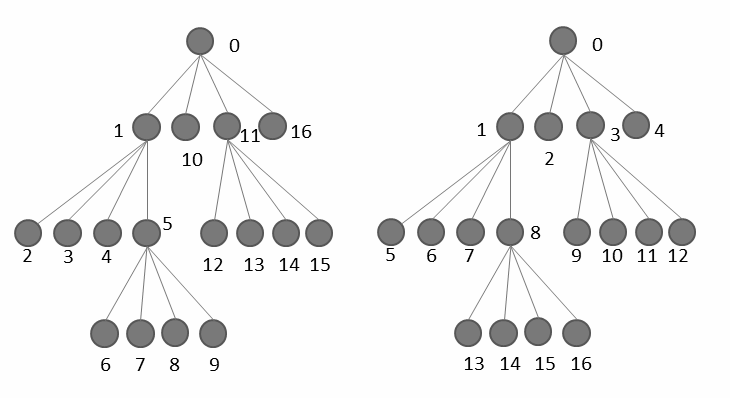
\includegraphics[width=12cm]{images/ch2/TreeTraversalExample}
\caption{Tree Traversals, Left: Depth First Traversal, Right Breadth First Traversal}
\label{TreeTraversalExample}
\end{figure}

Encoding the two packed tree traversal methods requires one nibble (4 bits) for a QT node, and one byte (8 bits) for an OT node. Here, the bits represent the structure of the sub-node. For example, the QT node bit sequence, $1001_2$ means that the node has two children (corresponding to the ones), the sequence $0000_2$ means the node is a leaf node. Each bit position indexes a child node using a pre-determined ordering. An example of a possible ordering for a quadrant and an octant is shown in figure \ref{ChildOrderExample}, both breadth-first and depth-first traversals use the same index method, the difference lies only in the order which nodes are visited. 

\begin{figure}[!htb]
\centering
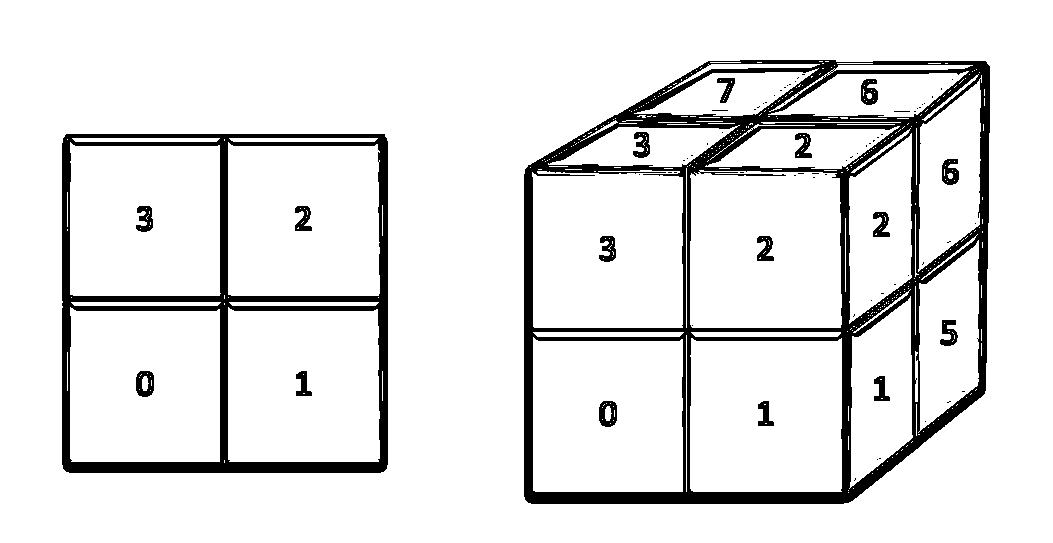
\includegraphics[width=12cm]{images/ch2/ChildOrderExample}
\caption{A possible child ordering for the QT (left), and the OT (right).}
\label{ChildOrderExample}
\end{figure}

The linear tree representation stores each leaf node individually. Each leaf is encoded as the pathway from the root to the leaf itself. This method was investigated in the 1980s \cite{Gargantini82Effective,Yufei88Octcodes}, but has not been used much in modern compression algorithms due to its inefficiency compared with the packed traversal method. An example of this structure is shown in figure \ref{LinearCellCodeRepresentation}, where each node: $a$, $b$, $c$, $\dots$ , $m$  is encoded as a variable length traversal path. The QT and OT are widely used in image \cite{Varma12Application} and 3D compression \cite{Schnabel06Octree}. Hanan Samet \cite{Samet88Fund1} presents an introduction to both of these structures, he also describes both tree storage methods in depth. 

\begin{figure}[!htb]
\centering
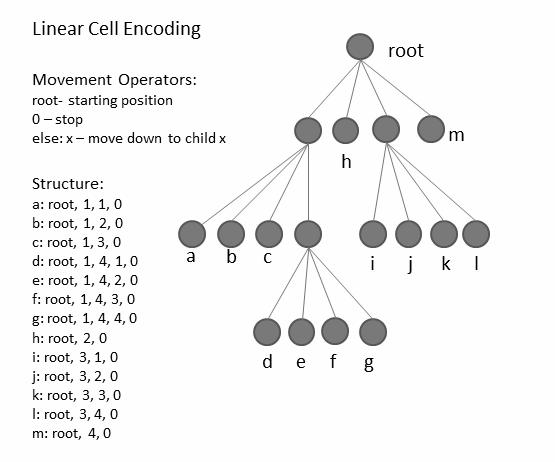
\includegraphics[width=12cm]{images/ch2/LinearCellCodeRepresentation}
\caption{A Linear Tree Code Representation Example}
\label{LinearCellCodeRepresentation}
\end{figure}



\subsection{3D ShadeTree Coding}

\label{sec:dr:coding}

The Shade-Tree compression system \ref{Gonzalez07ShadeTree} was designed for the compression of 2D image data. However, this method is easily extended to 3D Volumetric data. In this system, Octants are decomposed in the same manner as with a regular octree but the leaf node representation is different. In the Shade-Tree, the corner values in the volume are sampled for each node. Figure XXXXFFG shows an example of these corners given an Octree. The corner values are stored instead of the data within the cube. \\


The actual data representation is formed by interpolating between these 4 corner values to generate the data within the node. This representation saves space by storing 4 corner values only rather than the dense volumetric data. The method also boasts the ability for nodes to share data. For example, if two leaf nodes happen to share a corner we can simply encode the corner once using another data structure at the decompression stage at no cost to the representation. This is illustrated in figure FEFEEF. \\

This data representation may also be used to represent Signed Distance Functions, which are now commonly used in 3d reconstruction as a means of representation. In fact, such a scheme would greatly benefit the compression method of the Shade-Tree since its data is typically represented as smooth changes along a given path. 

\subsection{PlaneTree Coding}

Our method is based on octree subdivision, it begins by placing the mesh within a cube. It checks whether the the representation corresponding to this single cube is at a desired level of quality. If it is not, the cube is decomposed into 8 sub-cubes. For each sub-cube associated with the mesh, the process repeats. This process is typically controlled using an error threshold and a maximum depth value. At each level of subdivision, the error between the sub-cube (or node) representation of the space is compared to the part of the model within the cube. If the error is below the error threshold, decomposition stops. Likewise, if the level of subdivision is greater or equal to the maximum depth value, decomposition also stops. \\

In the typical octree node representation, the raw cube is used to represent the space. Unless this cube is small (deep within the tree) the error is typically high. Trees which are very deep require more storage space. Our method stores arbitrary first order planes within nodes at 20 bits per leaf. This small bit cost per leaf node greatly improves compression performance compared to the octree and makes it competitive with state of the art methods. \\

 
In the following sections, we present the details of the Plane-Tree in terms of subdivision, leaf node plane computation and representation as well as compression and decompression.


\subsection{Octree Subdivision}

Prior to compression, the input 3D model is normalized into a $512^3$ space. Starting with the cube which represents this space, we compute our 3D plane representation. Then the mean squared error between the sampled points of the plane and the sampled points of the model (which lie within the cube) is computed. If this value is below a given threshold, or the maximum level of subdivision is reached, decomposition stops. Alternatively if both of these predicates are not met, the cube is divided into 8 sub-cubes. Each sub-cube is then tested to see whether part of the mesh lies within it. If so, the process it repeated for that cube, otherwise no action is taken. \\

Each cube/sub-cube is referred to as a node. Each node which has no children is referred to as a leaf node. During compression/decompression, our plane based representation is only stored at leaf nodes, with non-leaf nodes serving only as paths giving the location of leaf nodes. Below, the computation and representation of our novel leaf node representation is discussed. \\

\subsection{Leaf Node Computation and Representation}
\label{NRep}
Our novel leaf node representation better represents the mesh which intersects it compared to the octree, it does so by using a first order plane. This representation requires only 20 bits, allowing us to achieve higher quality models whilst saving on bits which would otherwise be used to form a deeper, and thus more costly octree representation. It also gives our method an advantage at low bitrates. \\

In order to generate a plane for a given leaf node, we first sample the mesh within the node space. Using these points, the x, y and z axis variances are measured. These indicate how much variation lies across each axis within the node. We then find the plane using least squares, solving for the axis with the lowest variance. Once we have coefficients describing the plane, we use a single point on the plane, and the plane normal to describe it. \\

Using a point on the plane and a plane normal, we can find a set of triangles which represent the plane within the node. We first find all points in which the cube's edges intersect with the computed plane. Using the average point as the origin, and the plane's normal as the y-axis, we order the points based on their x/z angle. This gives us an ordered set of points which corresponds to a polygon defining the plane within the node. This polygon is then triangulated forming the final representation. This process is used at both the compression and decompression stages. \\

The triangles representing the plane within the node are then sampled along with the parts of the mesh lying within the node. The mean squared error (mse) is then taken between these samples for comparison with the error threshold value. Within the summation for the mse we use the closest point within the second point set, this is shown in equation \ref{eqn:MSE_1}.

\begin{equation}
 \label{eqn:MSE_1}
MSE(pts_1, pts_2) = \frac{1}{N}\sum_{i=0}^{N} (pts_{1_i} - closest(pts_{1_i}, pts_2))^2
\end{equation}

Using this equation and the sampled points from the plane triangles $p$, and the sampled points from the mesh $m$ (which lie within the cube), we take the average of both mean squared errors as a measurement of total error, $error = \frac{1}{2}MSE(p,m) + \frac{1}{2}MSE(m,p)$. This is the value which is compared with the error threshold to decide whether decomposition should stop or not. \\

In order to compress the data for our leaf node representation, we store the the plane using its normal vector and a single point lying on the plane. We store the normal vector using 12 bits (4 bits per coordinate). The point which lies on the plane is represented using two pieces of information, an edge number and a distance variable. First it must be mentioned that for a given plane which intersects a cube, a minimum of 3 of the cube's edges pass through the plane. We therefore record one of these edges (the edge number) and the distance from on of its end points (the distance variable). Each edge has a predefined number which identifies it, all edges also have a predefined start and end point. \\

Each cube has 12 edges in total, so 4 bits are used for the edge number, another 4 are used for the distance variable. Adding these to the normal vector totals to 20 bits per leaf node representation.  \\


\subsection{Compression and Decompression}

In order to compress our data structure we iterate through the tree in depth first order. If we encounter a non-leaf node, we first store a single bit of $1_2$. Then the configuration of the sub-nodes (since not every sub-node intersects the object) is stored as a single byte. Each bit is labelled $1_2$ if a particular sub-node exists and $0_2$ if it does not. This is possible since we order our sub-nodes in a predefined order. If a leaf node is encountered, we store a $0_2$, then record our 20 bit leaf node representation in three other files. One for the normal data, the distance variables and edge numbers totalling 4 files (tree, normals, distances and edge numbers). After the entire structure is stored we employ entropy encoding on each of these files. \\

In order to decompress our structure, we read the first bit of the output file. This checks if the current node is a leaf or not. If it is, we read out a 20 bit plane representation (from the three separate files) and generate a list of triangles representing where the plane intersects the node (explained in section \ref{NRep}). These triangles are then added to a final database which represents the decoded model. If we reach a non-leaf node, we read out the 8 bit sub-node configuration and repeat the process for each existing sub-nodes in the predefined order. \\  



\section{Conclusion}